\documentclass[10pt,twocolumn,a4paper]{article}

%% -- Typography & font -----------------------------------------------
\usepackage{times}
\usepackage{microtype}

%% -- Graphics ---------------------------------------------------------
\usepackage{epsfig}
\usepackage{graphicx}

%% -- Math -------------------------------------------------------------
\usepackage{amsmath}
\usepackage{amssymb}

%% -- Tables -----------------------------------------------------------
\usepackage{booktabs}
\usepackage{array}

%% -- Code listings ----------------------------------------------------
\usepackage{listings}
\usepackage{xcolor}

%% -- Page layout ------------------------------------------------------
\usepackage[a4paper, top=22mm, bottom=22mm, left=16mm, right=16mm]{geometry}
\setlength{\columnsep}{5mm}

\usepackage{float}
\usepackage{caption}
\usepackage{subcaption}
\usepackage{placeins}
\usepackage{stfloats}
\usepackage{balance}

%% -- Float placement parameters --------------------------------------
\setlength{\textfloatsep}{10pt plus 2pt minus 4pt}
\setlength{\floatsep}{8pt plus 2pt minus 4pt}
\setlength{\intextsep}{8pt plus 2pt minus 4pt}
\setlength{\dbltextfloatsep}{10pt plus 2pt minus 4pt}
\setlength{\dblfloatsep}{8pt plus 2pt minus 4pt}
\renewcommand{\topfraction}{0.90}
\renewcommand{\bottomfraction}{0.50}
\renewcommand{\textfraction}{0.07}
\renewcommand{\floatpagefraction}{0.85}
\renewcommand{\dbltopfraction}{0.90}
\renewcommand{\dblfloatpagefraction}{0.85}

%% -- Miscellaneous ----------------------------------------------------
\usepackage{csquotes}
\usepackage{hyperref}
\hypersetup{hidelinks}

%% -- Caption style ----------------------------------------------------
\captionsetup{font=small, labelfont=bf, skip=4pt}


\begin{document}

\title{\textbf{MFIN7092 Final Project}\\[4pt]
       Cross-Exchange Funding-Rate Arbitrage in Perpetual Futures:\\
       Form a Carry Illusion to a Capacity-Constrained, Risk-Calibrated Strategy}

\author{Cao Zhaoli\\[2pt]
        {\tt\small Student ID: 3036668420}\\[2pt]
        The Uiversity of Hong Kong}

\date{}

\maketitle
\thispagestyle{empty}

%% -- Abstract ---------------------------------------------------------
\begin{abstract}
I build a cross-exchange funding-rate arbitrage on 20 perpetual coins and six venues
foor one year.  The naive idea---rank coins by funding and trade the extremes---looks
like free money, but it loses money (full-PnL Sharpe $-2.54$) after I count the price
of every leg.  Many refinements, including a machine-learning model, all fail out of
sample.  Two delta-neutral strategies can work.  \textbf{Strategy A} (same coin, two
venues) gets an out-of-sample Sharpe of $2.34$ and can be used at any size.
\textbf{Strategy B} (negative cash-and-carry) reaches $7.47$ in regime, but it is off
78\% of the time and capped at \$130{,}926; an honest risk pipeline cuts it to a
single-year range of $[2.41, 3.81]$.  So A is the main, scalable strategy, and B is
only a small one.
\end{abstract}


%% =====================================================================
\section{Introduction}
\label{sec:intro}
%% =====================================================================

Perpetual futures (``perps'') are the main instrument in crypto trading.  A perp never
expires; instead the longs and the shorts pay each oher a regular \emph{funding}
rate, which keeps the perp price near the spot price (when the perp is above spot,
longs pay shorts, and below spot it is the opposite).  Funding on altcoin perps is
often large and stays for a long time, so it looks like easy carry.  Can I harvest it
in a systematic way?

The answer is no, at least not the naive way.  My main finding is negative: the simple
way to harvest funding does not only do worse, it \emph{loses money} after I count the
price risk honestly  So the rest of the report looks for a way to keep the funding
income but remove the prce risk.

My contributions is four.  First, I shhow that a funding-only PnL makes the Sharpe
look more than twenty points too high.  Second, I write down the failed ideas in an
open way.  Third, I build two delta-neutral strategies and split their Sharpe into
clear parts.  Fourth, I run a real-data risk pipeline that cuts Strategy~B's naive,
$7.47$ to an honest range and a hard cap.  The sections follow this order.


%% =====================================================================
\section{Background and Related Literature}
\label{sec:background}
%% =====================================================================

\subsection{The funding mechanism}
\label{sec:mechanism}

Let $P_t$ be the mark price and $I_t$ the spot index.  In each interval the exchange
sets a funding rate $f_t$, which is a pemium term plus an interest term,
\begin{equation}
  f_t \;\approx\; \text{clip}\!\Big(\tfrac{P_t - I_t}{I_t} + r^{\text{int}}_t,
       \; -\bar f,\; +\bar f\Big),
  \label{eq:funding_def}
\end{equation}
where $\bar f$ is the cap.  A long position of size $N$ gets the cash flow
\begin{equation}
  \pi^{\text{long}}_t = -f_t\,N, \qquad
  \pi^{\text{short}}_t = +f_t\,N ,
  \label{eq:funding}
\end{equation}
so a long collects funding when $f_t < 0$ and a short collects when $f_t > 0$.
\cite{ackerer2024perpetual} show that funding equals the cost of carry of a synthetic
spot-plus-financing position.  The key point is this: Equation~\eqref{eq:funding} is
\emph{only} the funding leg.  The total PnL of the perp also has a price term and a
cost term,
\begin{equation}
  \pi^{\text{total}}_t = \underbrace{-f_t N}_{\text{funding}}
                       + \underbrace{N\,\tfrac{P_{t+1}-P_t}{P_t}}_{\text{price}}
                       - \underbrace{c_t}_{\text{cost}} .
  \label{eq:total}
\end{equation}
So if a strategy reports only the funding term, the, number is not real, unless the
price term is already removed in another way.

\subsection{Perpetual pricing and the basis}

Define the basis $b_t = (P_t - I_t)/I_t$.  Two facts are useful.  The same-coin
same-venue basis (a perp against its own spot) is small and mean-reverts, so a
single-venue hedge is clean---this is the base of Strategy~B.  The same-coin
cross-venue basiis (one exchange's perp against another's) is larger and slower,
because to close it I need capital on two venus at the same time
\cite{makarov2020trading}---this is the base of Strategy~A.

\subsection{Carry, dispersion and the cross-section}

Three lines of literature shape the design.  The \emph{carry} line
\cite{schmeling2023crypto} treats funding as a risk premium that depends on the state.
The \emph{arbitrage and dispersion} line \cite{makarov2020trading} shows that
cross-exchange gaps mean-revert but are limited by how fast capital can move.  The
\emph{factor} line \cite{liu2022common, borri2022cross} prices the cross-section, and
I use it as a benchmark.  I also use \cite{moreira2017volatility} for sizing
\cite{almgren2001optimal} for cost, \cite{foucault2017toxic} and
\cite{bailey2014deflated} for honest testing, \cite{sebastiao2021forecasting} for the
ML part, and \cite{hu2023crypto} for crowding.

\subsection{Funding as a price of leverage}

Funding is the interest of leverage: a long perp is a spot long with leverage, and
without frictions funding would be near the risk-free rate \cite{ackerer2024perpetual}.
The large and often \emph{negative} funding I find (Section~\ref{sec:eda}) is the gap
from this benchmark, and its size shows how strong the frictions are.  Negative
funding means traders are willing to pay to be short, that is, the natural longs are
too few.  So to harvest funding is to give missing this leverage---it is a paid risk,
not a free profit.

\subsection{How this paper relates to prior work}

Most crypto-arbitrage papers study the \emph{price} gap across venues
\cite{makarov2020trading}.  Strategy~A moves this idea to the \emph{funding} basis: I
trade the slow and lasting cross-venue funding difference, not thhe fast price gap.  So
the contribution of this paper is not a new anomaly, but a careful, friction-aware
build and de-risk of two usable strategies, with an honest count of how much edge is
left after price risk, borrow limit, and regime.


%% =====================================================================
\section{Methodology: Data and Backtest Engine}
\label{sec:method}
%% =====================================================================

\subsection{Data}

Table~\ref{tab:data} lists the inputs: an Auros funding feed (about 365{,}000 events),
65~GB of Tardis tick data put into a 4-hour panel, OKX and Gate.io spot, and live OKX
borrow rates annd quotas.

\begin{table}[htbp]
  \centering
  \caption{\textbf{Data sources and roles.}}
  \label{tab:data}
  \begin{tabular}{lll}
    \toprule
    \textbf{Input} & \textbf{Source} & \textbf{Role} \\
    \midrule
    Funding history   & Auros feed        & primary signal \\
    Derivative ticker & Tardis (65\,GB)   & mark / OI / basis \\
    Spot prices       & OKX, Gate.io API  & cash-and-carry \\
    Borrow / quota    & OKX lending API   & B financing $+$ cap \\
    Fees              & VIP9 schedules    & cost model \\
    \bottomrule
  \end{tabular}
\end{table}

The uiverse is 20 coins on six venues (Binance, Bybit, Gate.io, Hyperliquid, KuCoin,
OKX), which gives 118 coin-venue pairs.  These coins survived six to twelve months, so
there is a survivorship bias, and I measure its cost in Section~\ref{sec:risk}.

\subsection{The 4-hour decision grid}

Funding setltes on different clocks (from hourly to 8-hourly), so I use a 4-hour grid
that lets every venue fall on a bin edge.  To avoid look-ahead, the funding I collect
in a bin is set just before the, bin ends so the rate I see when I decide is never the
rate that pays.  The out-of-sample (OOS) period is the lsat six months (1{,}086 bins);
the first six months are in-sample, for any parameter I must choose.

\subsection{The backtest engine}

All strategies usse one engine.  At each bin it computes a signal chooses positions,
and holds them with a \emph{stickiness} rule: a position opens only above an entry
threshold $\theta_{\text{ent}}$, and closes only below an eit threshold
$\theta_{\text{ext}} < \theta_{\text{ent}}$, which is the toxic-arbitrage buffer of
\cite{foucault2017toxic}.  The sizing follows \cite{moreira2017volatility},
\begin{equation}
  w_{i,t} \;=\; \text{clip}\!\Big(\frac{v^\star}{\hat\sigma_{i,t}},
              \; w_{\min},\; w_{\max}\Big),
  \label{eq:voltarget}
\end{equation}
with $v^\star = 150$~bp, $w_{\min}=0.3$, $w_{\max}=1.5$, and $\hat\sigma_{i,t}$ lagged
by one bin.

\subsection{Cost and fill model}

Every leg pays the VIP9 maker fee plus 1~bp slippage, and I count the, round-trip cost
only when a possition changes,
\begin{equation}
  c_t \;=\; \sum_{i \in \Delta_t}\big(\text{maker}_{e(i)} + 1\,\text{bp}\big),
  \label{eq:cost}
\end{equation}
where $\Delta_t$ is the legs opened or closed at $t$.  Fills are a probability, not a
sure thing: a signalled entry is taken with probability $0.8$, and the entry-bin price
PnL is cut by 12.5\%.  All Sharpe ratios are after cost and are annualised with
$\sqrt{365\cdot 24/4}$.

\subsection{Evaluation philosophy}

The main number is the annualised Sharpe,
\begin{equation}
  \text{Sh} \;=\; \frac{\bar r}{\hat\sigma_r}\,\sqrt{N_{\text{yr}}},
  \qquad N_{\text{yr}} = \frac{365\cdot 24}{4}.
  \label{eq:sharpe}
\end{equation}
Two choices come again and again.  For an on-off strategy (B) I report a bootstrapped
\emph{range}, not one point, because the in-regime Sharpe is not what a live book
earns.  For any regression I use Newey--West errors \cite{newey1987simple}, because
funding and basis are autocorrrelated.

\subsection{Look-ahead controls and validation}

Overfitting can come from three doors, and I close each one.  \emph{Future
information}: every signal uses only data before $t$ (the collected funding, the
lagged volatility, and the forward price).  \emph{Parameter selection}: I choose
parameters on the first six months only, and report all results on the untouched last
six months.  \emph{Survivorship}: Section~\ref{sec:risk} adds phantom delistings at a
live-measured rate.  Because I tried many variants, I treat the winners as upper
bounds and report the deflated Sharpe \cite{bailey2014deflated}.


%% =====================================================================
\section{Exploratory Data Analysis}
\label{sec:eda}
%% =====================================================================

First I look at teh funding data, because its shape decides which strategies can work

\subsection{The shape of funding}

Figure~\ref{fig:funddist} shows a sharp peak at zero and a heavy negative taail, so a
few coins carry most of the money---this is where Strategy~B lives.

\begin{figure}[htbp]
  \centering
  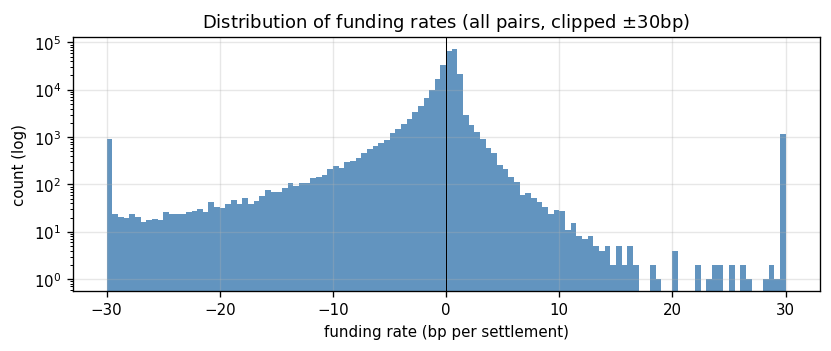
\includegraphics[width=\linewidth]{figures/eda_funding_dist.png}
  \caption{\textbf{Distribution of funding rates.}  Pooled across all 118 pairs
           (clipped to $\pm$30~bp, log count axis).  A sharp zero-peak with a
           heavy negative tail---the negative tail is where Strategy~B lives.}
  \label{fig:funddist}
\end{figure}

Table~\ref{tab:fundcoin} splits this by coin.  The large caps have small positive
funding and no carry; the mid-caps and meme coins (BERA, KAIITO, IP, MOODENG) stay
deeply negative adn pay a long a large yearly subsidy.  This is the reason for
Strategy~B.

\begin{table}[htbp]
  \centering
  \caption{\textbf{Funding summary statistics by coin (per settlement).}}
  \label{tab:fundcoin}
  \begin{tabular}{lrrr}
    \toprule
    \textbf{Coin} & \textbf{Mean (bp)} & \textbf{Std (bp)} & \textbf{Neg (\%)} \\
    \midrule
    BTC     & $+0.32$ & 0.56  & 21.6 \\
    ETH     & $+0.28$ & 0.69  & 27.0 \\
    LTC     & $+0.35$ & 0.86  & 24.6 \\
    DOGE    & $+0.34$ & 1.30  & 26.9 \\
    SOL     & $+0.07$ & 1.52  & 38.8 \\
    AVAX    & $+0.06$ & 1.68  & 36.7 \\
    TAO     & $+0.10$ & 1.64  & 25.3 \\
    POPCAT  & $+0.21$ & 1.83  & 18.6 \\
    WLD     & $+0.11$ & 1.65  & 31.9 \\
    TIA     & $-0.01$ & 1.68  & 32.5 \\
    JUP     & $-0.13$ & 1.34  & 38.1 \\
    TRUMP   & $-0.29$ & 2.23  & 45.3 \\
    JTO     & $-0.27$ & 5.38  & 28.0 \\
    MOODENG & $-1.29$ & 5.72  & 41.0 \\
    IP      & $-2.01$ & 7.04  & 53.4 \\
    KAITO   & $-2.47$ & 10.74 & 51.3 \\
    BERA    & $-3.42$ & 9.50  & 75.7 \\
    PIPPIN  & $+19.1$ & 52.3  & 12.6 \\
    \bottomrule
  \end{tabular}
\end{table}

\subsection{Funding differs across venues}

Funding also differs across venues for the same coin, and this is the raw material of
Strategy~A.  In Table~\ref{tab:fundexch} OKX is special (mean $+3.59$~bp, spread
$24.6$~bp), while KuCoin is negative for mre than half the time.

\begin{table}[htbp]
  \centering
  \caption{\textbf{Funding summary statistics by exchange.}}
  \label{tab:fundexch}
  \begin{tabular}{lrrr}
    \toprule
    \textbf{Exchange} & \textbf{Mean (bp)} & \textbf{Std (bp)} & \textbf{Neg (\%)} \\
    \midrule
    Binance     & $-0.60$ & 5.25  & 36.7 \\
    Bybit       & $-0.19$ & 4.43  & 26.4 \\
    Gate.io     & $-0.45$ & 5.67  & 29.4 \\
    Hyperliquid & $-0.11$ & 1.19  & 30.6 \\
    KuCoin      & $-0.86$ & 5.96  & 52.8 \\
    OKX         & $+3.59$ & 24.56 & 31.9 \\
    \bottomrule
  \end{tabular}
\end{table}

Figures~\ref{fig:heatmap} and~\ref{fig:venuecorr} show that, coins differ (rows) and
venues differ (columns), and that venues move together but are not the same.  Teh left
gap closes only slowly \cite{makarov2020trading}.

\begin{figure}[htbp]
  \centering
  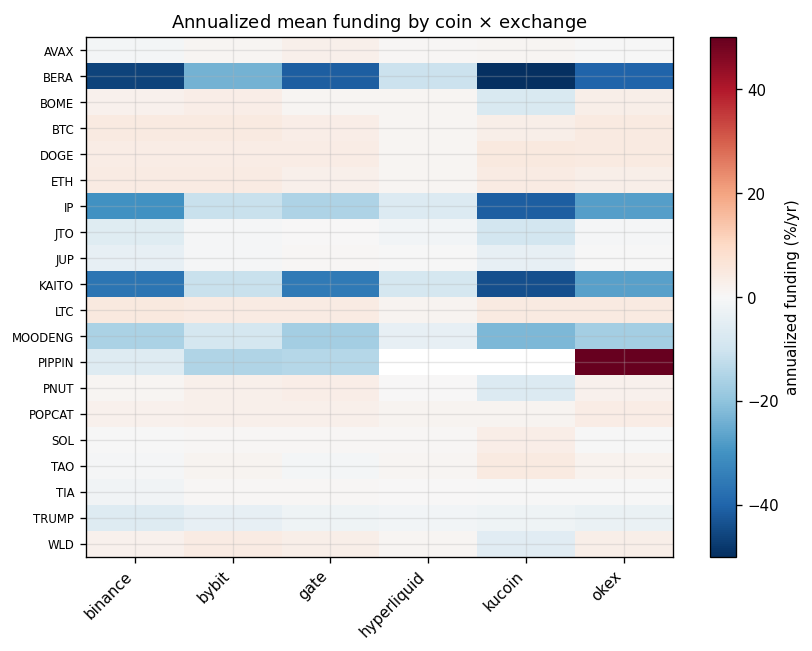
\includegraphics[width=\linewidth]{figures/eda_funding_heatmap.png}
  \caption{\textbf{Annualised funding by coin $\times$ exchange.}  Coins differ
           (rows) and venues differ (columns); the within-row variation is the
           spread Strategy~A trades.}
  \label{fig:heatmap}
\end{figure}

\begin{figure}[htbp]
  \centering
  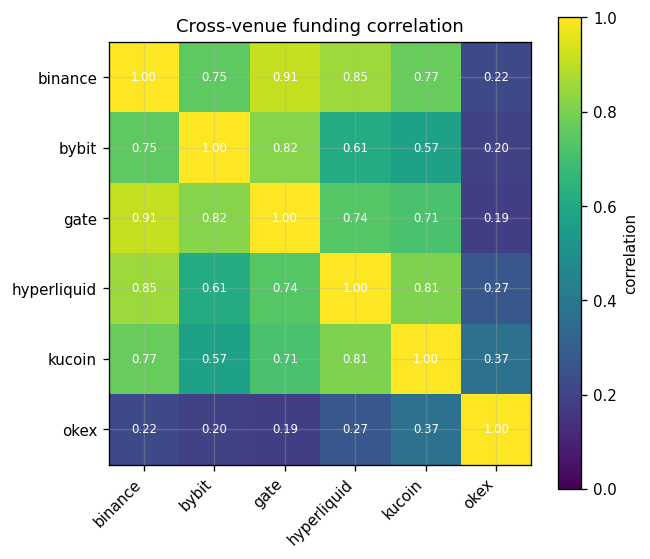
\includegraphics[width=\linewidth]{figures/eda_venue_corr.png}
  \caption{\textbf{Cross-venue funding correlation.}  Venues move together but are
           far from the same; the leftover difference is what a same-coin pair
           earns.}
  \label{fig:venuecorr}
\end{figure}

\subsection{Persistence: why ML is useless}

Funding changes very slowly: the lag-1 (4-hour) autocorrelation is $0.57$, and it is
still $0.27$ one day later (Table~\ref{tab:persist}, Figure~\ref{fig:persist}).  So
the simple forecast ``next $=$ current'' is hard to beeat, and a model cannot help
(Section~\ref{sec:failed}: OOS $R^2$ $0.70$ foor the simple rule against $0.23$ for
LightGBM).

\begin{table}[htbp]
  \centering
  \caption{\textbf{Funding persistence (cross-pair mean ACF).}}
  \label{tab:persist}
  \begin{tabular}{lr}
    \toprule
    \textbf{Lag} & \textbf{Autocorrelation} \\
    \midrule
    1 (4h)   & 0.571 \\
    3 (12h)  & 0.345 \\
    6 (24h)  & 0.268 \\
    12 (48h) & 0.188 \\
    24 (96h) & 0.134 \\
    \bottomrule
  \end{tabular}
\end{table}

\begin{figure}[htbp]
  \centering
  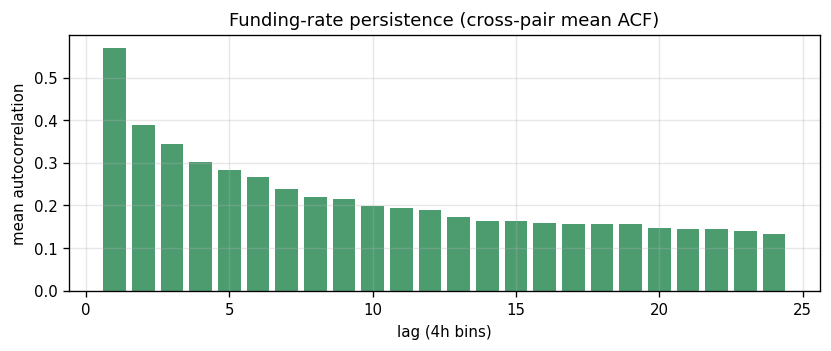
\includegraphics[width=\linewidth]{figures/eda_persistence.png}
  \caption{\textbf{Funding-rate persistence.}  The autocorrelation starts at
           $0.57$ and falls slowly.  This explains why funding is harvestable and
           why a model cannot beat the simple forecast.}
  \label{fig:persist}
\end{figure}

\subsection{The cross-exchange spread is large and frequent}

Strategy~A trades the cross-exchange funding spread $g$.  Its median is $8.8$~bp and
its 99th percentile is $15.9$~bp (Table~\ref{tab:spread}), both well above the $3$~bp
entry threshold, so it fires often; it also widens in stress
(Figure~\ref{fig:spread}).

\begin{table}[htbp]
  \centering
  \caption{\textbf{Cross-exchange funding-spread percentiles (bp).}}
  \label{tab:spread}
  \begin{tabular}{lrrrrr}
    \toprule
    & \textbf{p50} & \textbf{p75} & \textbf{p90} & \textbf{p95} & \textbf{p99} \\
    \midrule
    Spread & 8.8 & 9.8 & 10.8 & 11.9 & 15.9 \\
    \bottomrule
  \end{tabular}
\end{table}

\begin{figure}[htbp]
  \centering
  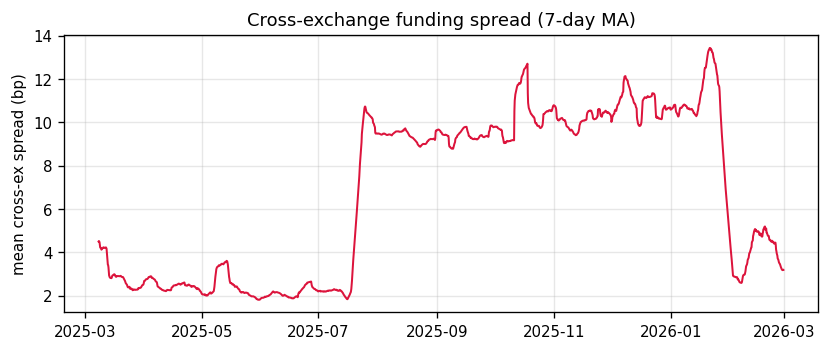
\includegraphics[width=\linewidth]{figures/eda_xex_spread.png}
  \caption{\textbf{Cross-exchange funding spread over time (7-day MA).}  The
           spread stays above Strategy~A's 3~bp entry threshold and widens in
           stressed periods.}
  \label{fig:spread}
\end{figure}

\begin{figure}[htbp]
  \centering
  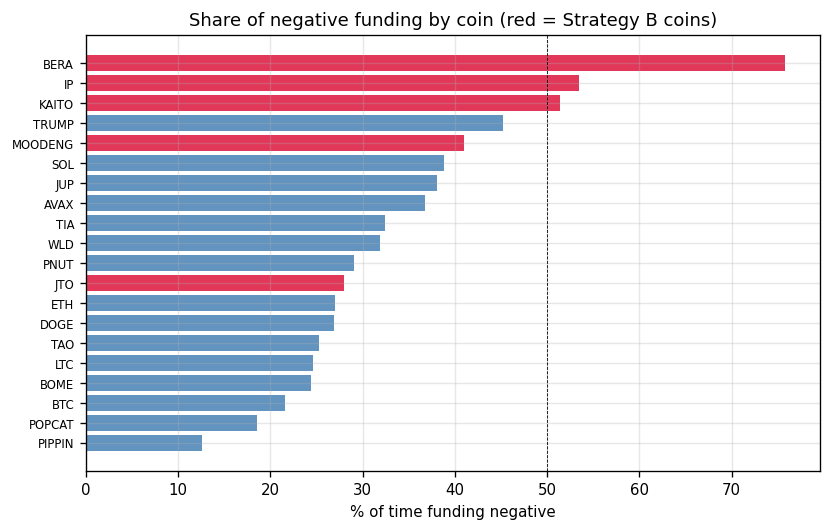
\includegraphics[width=\linewidth]{figures/eda_neg_share.png}
  \caption{\textbf{Share of negative funding by coin.}  Strategy~B's five coins
           (red) are negative far more often than the majors, so the
           cash-and-carry edge lives in the mid-cap/meme group.}
  \label{fig:negshare}
\end{figure}

Figure~\ref{fig:negshare} confirms the coin choice: Strategy~B's five coins is
negative most often.

\subsection{Funding paths through time}

Figure~\ref{fig:fundts} shows that BTC stays near zero, while KAITO and BERA stay
deeply negative for long times and then jump back.  So the carry is on-off, not
constant---this is the root of the regime risk in Section~\ref{sec:risk}.

\begin{figure}[htbp]
  \centering
  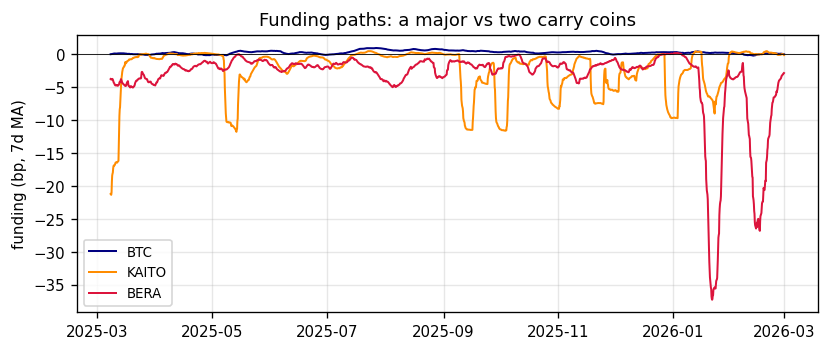
\includegraphics[width=\linewidth]{figures/eda_funding_ts.png}
  \caption{\textbf{Funding paths: a major versus two carry coins.}  BTC stays near
           zero; KAITO and BERA spend long episodes deeply negative.  The carry is
           on-off, the root of the regime risk in Section~\ref{sec:risk}.}
  \label{fig:fundts}
\end{figure}

\subsection{Liquidity: open interest}

Depth differs by orders of magnitude (Figure~\ref{fig:oi}).  This is why Strategy~A
uses only the eight most liquid coins, and why Strategy~B's thin mid-caps make its
size only tens of thousands of dollars.

\begin{figure}[htbp]
  \centering
  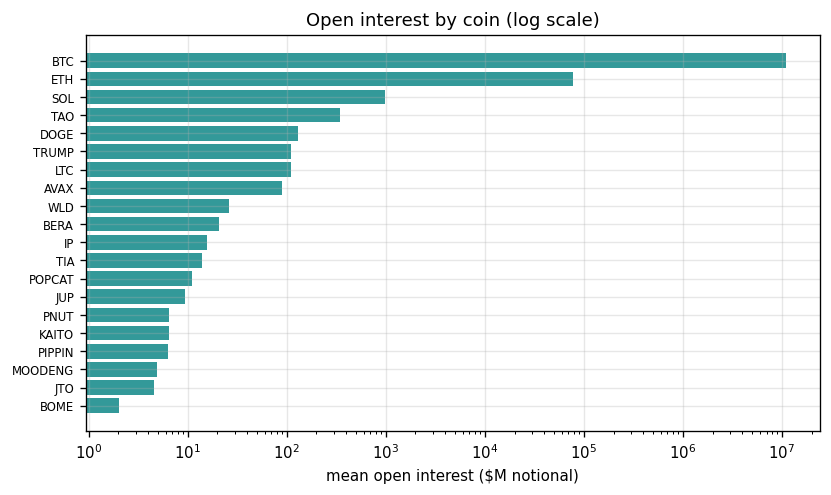
\includegraphics[width=\linewidth]{figures/eda_oi.png}
  \caption{\textbf{Open interest by coin (log scale).}  Depth spans several orders
           of magnitude; this gradient sets which coins each strategy can trade
           and at what size.}
  \label{fig:oi}
\end{figure}

\subsection{The basis}

Over all pairs, the mark-minus-index basis has mean, $-5.3$~bp and standard deviation
$13.7$~bp (Figure~\ref{fig:basis}); this spread makes the basis tradeable, and its
mean reversion is the second engine of Strategy~A.

\begin{figure}[htbp]
  \centering
  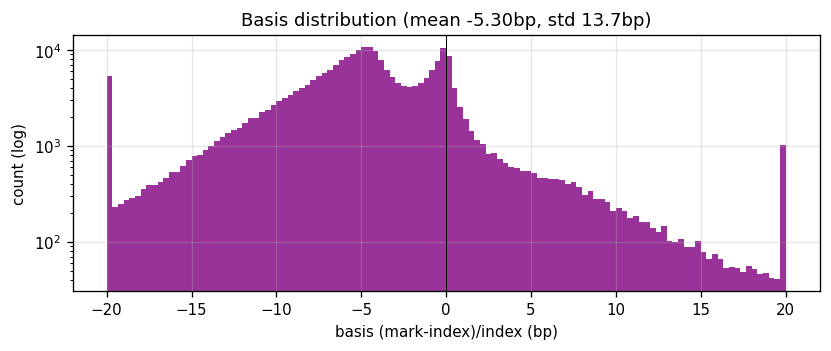
\includegraphics[width=\linewidth]{figures/eda_basis.png}
  \caption{\textbf{Basis distribution (mark $-$ index).}  Mean $-5.3$~bp, standard
           deviation $13.7$~bp, with heavy tails; the spread is the raw material of
           the basis-convergence engine.}
  \label{fig:basis}
\end{figure}

\subsection{Intraday seasonality}

There is a small hour-of-day pattern (Figure~\ref{fig:season}), but it is small next
to the cross-sectional and regime variation, so I do not use it.

\begin{figure}[htbp]
  \centering
  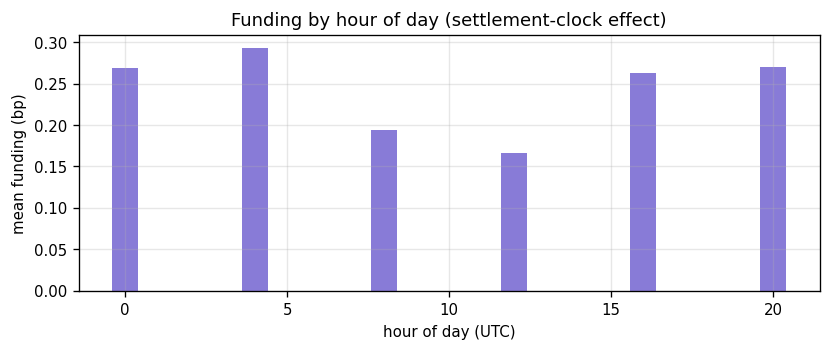
\includegraphics[width=\linewidth]{figures/eda_seasonality.png}
  \caption{\textbf{Funding by hour of day (UTC).}  A mild settlement-clock pattern
           exists but is small next to the cross-sectional and regime variation the
           strategies use.}
  \label{fig:season}
\end{figure}

\subsection{Mean reversion: what is tradeable}

Figure~\ref{fig:halflife} compares two things.  The fundng spread lasts (lag-1
$0.57$, half-life about $5$~h), so I can catch it on a 4-hour grid.  The price basis
reverts almost at once (lag-1 $-0.04$, half-life under $15$~min), so to trade the
cross-exchange \emph{price} gap direcctly is hopeless.  So Strategy~A trades the lasting
funding spread, not the price gap.

\begin{figure}[htbp]
  \centering
  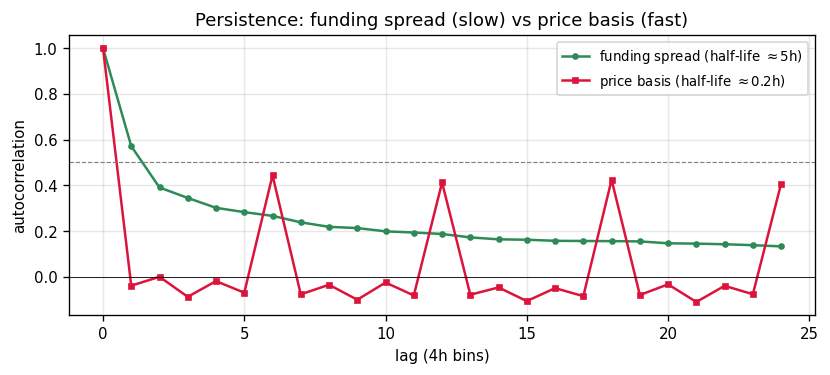
\includegraphics[width=\linewidth]{figures/eda_halflife.png}
  \caption{\textbf{Persistence: funding spread versus price basis.}  The funding
           spread reverts slowly (half-life $\approx 5$~h, tradeable); the price
           basis reverts almost at once (half-life $<15$~min, untradeable).
           Strategy~A trades the funding spread.}
  \label{fig:halflife}
\end{figure}


%% =====================================================================
\section{The Funding-Carry Illusion: A Na\"ive Baseline}
\label{sec:baseline}
%% =====================================================================

The first obvious trade ranks all 118 pairs by funding and trades the extremes: long
the 24 most-negative, short the 24 most-positive, equal weight, no hedge.  On the
\emph{full} PnL of Equation~\eqref{eq:total}, it fails (Figure~\ref{fig:baseline}): the
funding part goes up ($+0.38$), but the unhedged price part loses a lot ($-0.79$), so
the Sharpe is $\mathbf{-2.54}$ and the return is $-90\%$ a year.

\begin{figure}[htbp]
  \centering
  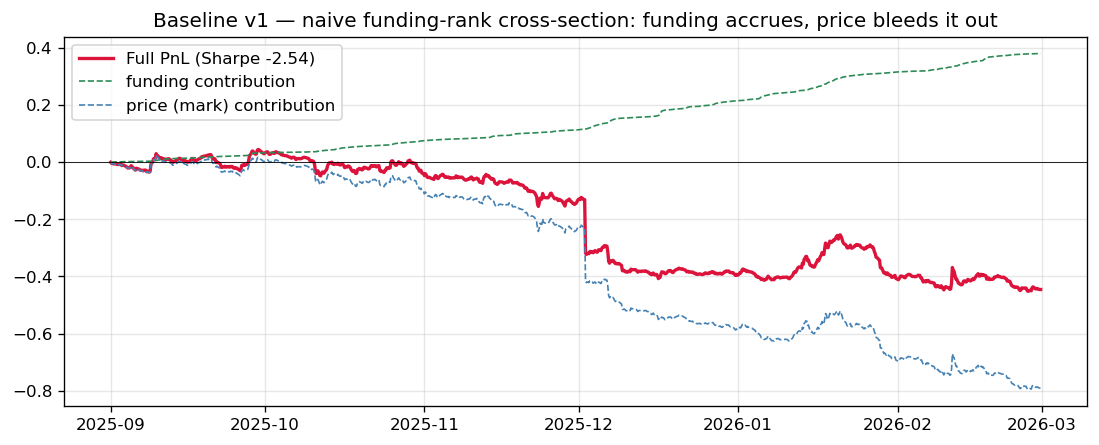
\includegraphics[width=\linewidth]{figures/final_01_baseline.png}
  \caption{\textbf{Na\"ive funding-rank cross-section (full PnL).}  Funding
           accrues steadily (green), but the unhedged price term (blue) dominates
           and the net book (red) loses: Sharpe $-2.54$.}
  \label{fig:baseline}
\end{figure}

The reason is simple.  The long leg, and the short leg are \emph{different coins}, so
the book is not market-neutral; its cross-sectional variance is one to two orders of
magnitude larger than the small funding it wants to collect.  If I report only the
funding term the Sharpe looks above $+27$, but ths is not real.  So the rest of the
report keeps the funding but removes the price---across venues (A) or against spot
(B).


%% =====================================================================
\section{A Catalogue of Failed Attempts}
\label{sec:failed}
%% =====================================================================

Before the sttrategies that work, I write down the ones that fail, because a process
that reports only winners looks the same as overfitting.

\subsection{Machine-learning funding prediction}

I used LightGBM to predict the next funding \cite{sebastiao2021forecasting}.  It lost
to the simplest forecast: OOS $R^2 = 0.23$ against $0.70$ for ``next $=$ current''.
Funding chnages too solwly for a model to add anythinng, so I dropped it.

\subsection{Universe expansion and the look-ahead trap}

To add more coins by an open-interest cutoff seemed to help (Sharpe $3.09$), but only
wheen I chose the cutoff on the full sample; when I chose it on training the window
only, it feell to $1.82$.  So the gaap was pure look-ahead.

\subsection{Fifteen microstructure and sizing variants}

I tested fifteen more ideas (Table~\ref{tab:coldlist}): threshold tiers, gap sizing,
an AR(1) predictor, toxic-move and crowing filters
\cite{foucault2017toxic, hu2023crypto}, sign rules, top-$K$, persistence gates, and
volatility swaps.  None of them clearly beat the Strategy~A baseline out of sample.  So
the edge is in the structure, not in the add-ons.

\begin{table}[htbp]
  \centering
  \caption{\textbf{The cold list: fifteen rejected variants (strict OOS Sharpe).}}
  \label{tab:coldlist}
  \begin{tabular}{lr}
    \toprule
    \textbf{Variant} & \textbf{Sharpe} \\
    \midrule
    Tier-scaled threshold (T1$=$1.5bp, T2$=$3bp) & 1.60 \\
    Position size $\propto \sqrt{\text{gap}}$      & 1.66 \\
    Position size $\propto$ gap (linear)           & 1.74 \\
    AR(1) basis prediction (enter early)           & 0.66 \\
    Toxic-move filter \cite{foucault2017toxic}     & 1.66 \\
    OI z-score $>2$ skip \cite{hu2023crypto}       & 1.82 \\
    Require sign reversal                          & 1.53 \\
    Top-$K$ cross-section                          & 1.83 \\
    Signal persistence ($k=2$ bins)               & 0.98 \\
    EWMA vol replacement (24h)                     & 1.93 \\
    Rolling-48h vol replacement                    & 1.87 \\
    Regime-adaptive threshold                      & 1.60 \\
    BTC delta hedge (already neutral)              & 2.34 \\
    Positive cash-and-carry                        & $-$1.15 \\
    Multi-stream tangency                          & 2.40 \\
    \bottomrule
  \end{tabular}
\end{table}

\subsection{Positive cash-and-carry}

The opposite positive cash-and-carry had an OOS Sharpe of $-1.15$: in this, sample only
the negative-funding side paid, and this side became Strategy~B.
Figure~\ref{fig:rejected} shows that none of the rejected curves pulls away.

\begin{figure}[htbp]
  \centering
  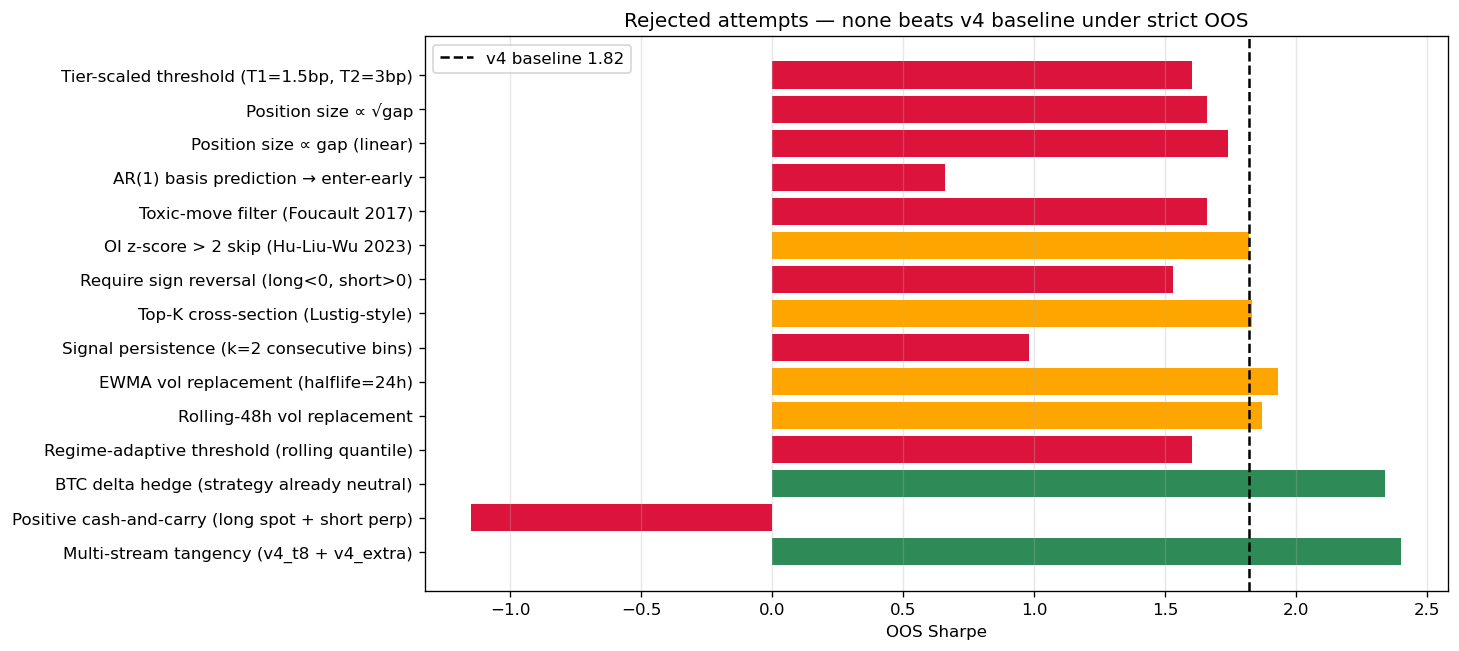
\includegraphics[width=\linewidth]{figures/final_02_rejected.png}
  \caption{\textbf{Rejected variants.}  Equity curves of the main failed ideas.
           None gave a robust, scalable gain over the simple delta-neutral pair of
           Section~\ref{sec:stratA}.}
  \label{fig:rejected}
\end{figure}


%% =====================================================================
\section{Strategy A: Cross-Exchange Funding-Spread Capture}
\label{sec:stratA}
%% =====================================================================

\subsection{Construction}

Strategy~A keeps the funding income but removes the price, by trading the \emph{same
coin} on two venues  For each coin I watch the cross-exchange spread
$g = \max_e f_{e} - \min_e f_{e}$.  When $g \ge 3$~bp I opn a delta-neutral pair: I
long the perp on the lowest-funding venue (it pays me as a long) and short the perp on
the highest-funding venue (it pays me as a short).  Because both legs are the same
coin, the price cancels, and what is left is the funding difference plus a small
cross-exchange basis that mean-reverts \cite{makarov2020trading}.  I hold unitl the
spread turns over or a $1.5$~bp exit \cite{foucault2017toxic}, size by
Equation~\eqref{eq:voltarget}, and use only the eight most liquid coins.

\subsection{Performance}

In the six-month OOS window, Strategy~A gets a Sharpe of $\mathbf{2.34}$, $8.8\%$ a
year, $3.7\%$ volatility, and a max drawdown of only $-0.9\%$ (Table~\ref{tab:headline},
Figure~\ref{fig:Aequity})---a stable relative-value profile, the opposite of the
baseline.

\begin{table}[htbp]
  \centering
  \caption{\textbf{Headline performance (OOS).}}
  \label{tab:headline}
  \begin{tabular}{lrrrr}
    \toprule
    \textbf{Strategy} & \textbf{Sharpe} & \textbf{Ann.\ Ret} & \textbf{Vol} & \textbf{MDD} \\
    \midrule
    Baseline v1 (na\"ive)   & $-2.54$ & $-90\%$  & ---    & ---     \\
    Strategy A (v4)         & $+2.34$ & $+8.8\%$ & 3.7\%  & $-0.9\%$ \\
    Strategy B (in-regime)  & $+7.47$ & $+190\%$ & 25.5\% & $-5.0\%$ \\
    \bottomrule
  \end{tabular}
\end{table}

\begin{figure}[htbp]
  \centering
  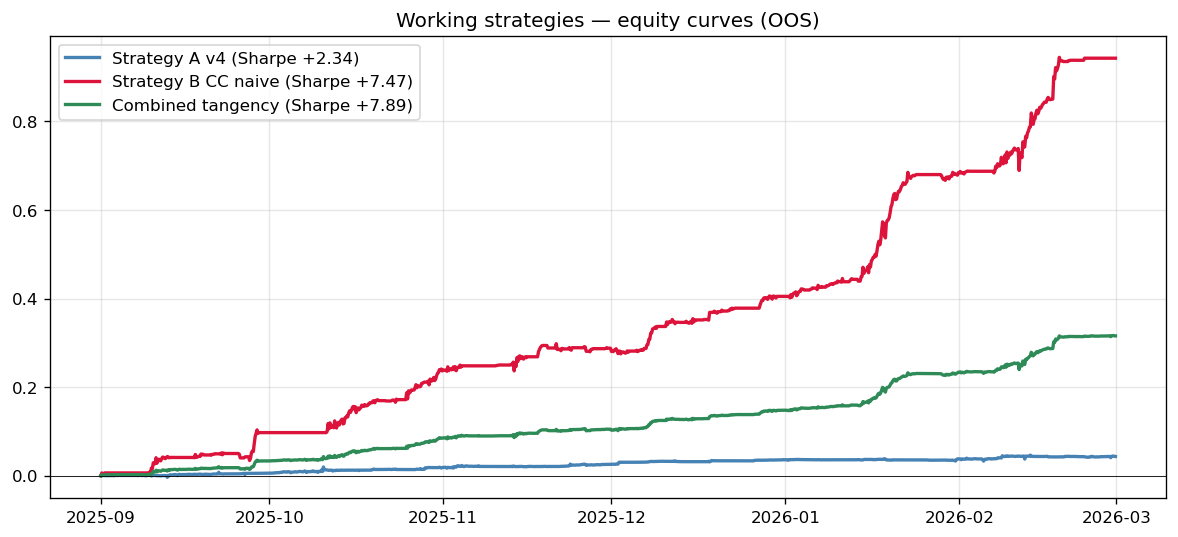
\includegraphics[width=\linewidth]{figures/final_03_working_equity.png}
  \caption{\textbf{Strategy A equity (OOS).}  The delta-neutral cross-exchange pair
           grows smoothly to a Sharpe of $2.34$ with a maximum drawdown of
           $-0.9\%$.}
  \label{fig:Aequity}
\end{figure}

\subsection{The two engines}

Figure~\ref{fig:Adecomp} splits teh PnL into funding and basis: the two parts are
about the samme size and almost independent, so when one engine is quiet, the other one
often is not.

\begin{figure}[htbp]
  \centering
  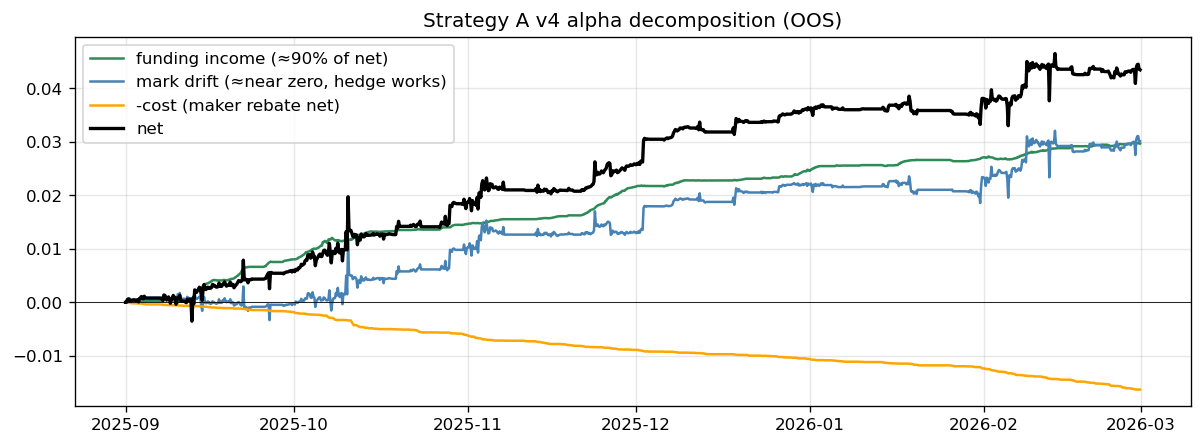
\includegraphics[width=\linewidth]{figures/final_04a_v4_decomposition.png}
  \caption{\textbf{Strategy A: funding versus cross-exchange basis.}  The two parts
           are about the same size and almost independent---two engines, not one.}
  \label{fig:Adecomp}
\end{figure}

\subsection{Sizing}

Volatility-target sizing adds about half a Sharpe point (Figure~\ref{fig:Asizing}),
because it sizes up when the pair is calm and down when it is wild.

\begin{figure}[htbp]
  \centering
  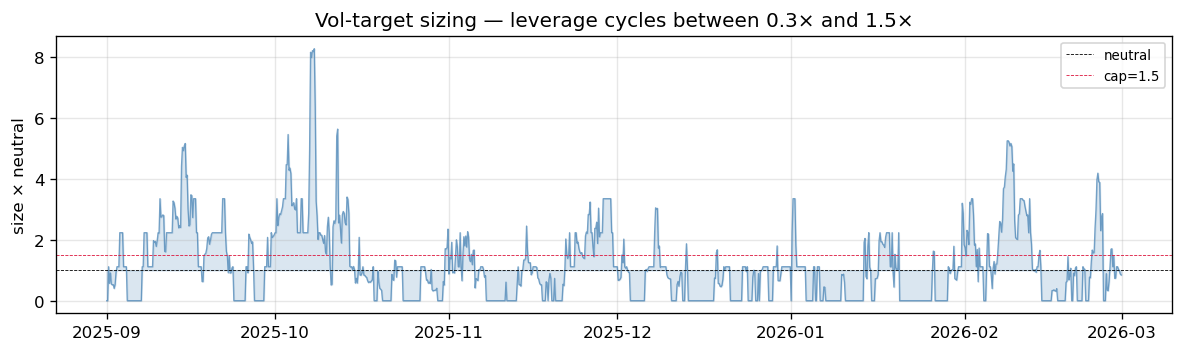
\includegraphics[width=\linewidth]{figures/final_04b_vol_target_sizing.png}
  \caption{\textbf{Volatility-target sizing.}  Scaling against volatility (target
           150~bp, cap $1.5\times$) adds about $+0.5$ Sharpe by cutting exposure
           when pair volatility spikes.}
  \label{fig:Asizing}
\end{figure}

\subsection{Stability and return profile}

Three more checks support the stability: the 30-day rolling Sharpe stays positive
(Figure~\ref{fig:Aroll}), the worst drawdown is $-0.9\%$ with fast recovry
(Figure~\ref{fig:Add}), and most months are positive (Figure~\ref{fig:Amonthly}).

\begin{figure}[htbp]
  \centering
  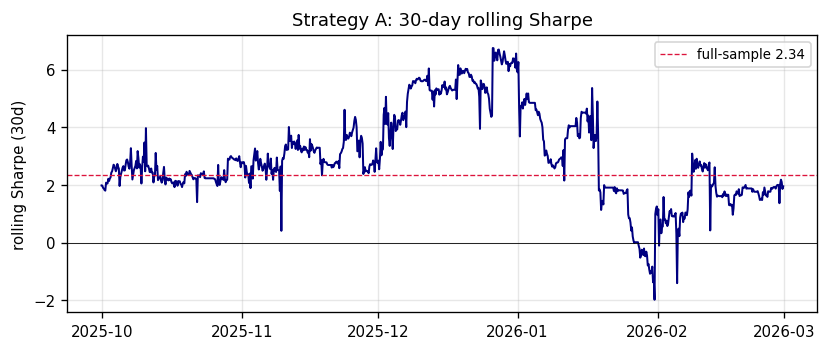
\includegraphics[width=\linewidth]{figures/an_A_rolling_sharpe.png}
  \caption{\textbf{Strategy A: 30-day rolling Sharpe.}  The rolling value stays
           positive and moves around the full-sample $2.34$ (dashed): the edge is
           steady, not a one-off.}
  \label{fig:Aroll}
\end{figure}

\begin{figure}[htbp]
  \centering
  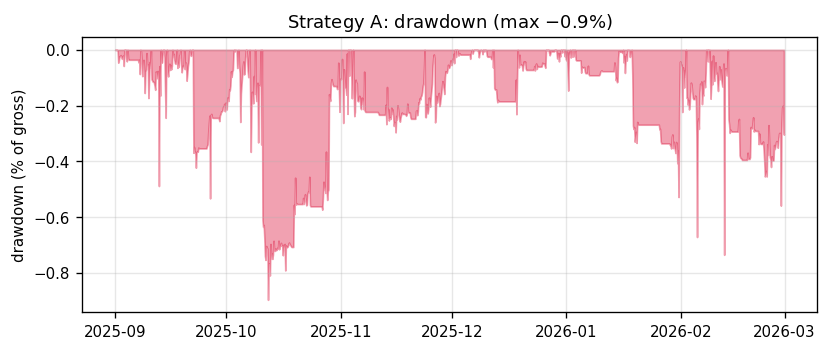
\includegraphics[width=\linewidth]{figures/an_A_drawdown.png}
  \caption{\textbf{Strategy A: drawdown.}  The maximum drawdown is $-0.9\%$ with
           fast recoveries---the sign of a relative-value trade.}
  \label{fig:Add}
\end{figure}

\begin{figure}[htbp]
  \centering
  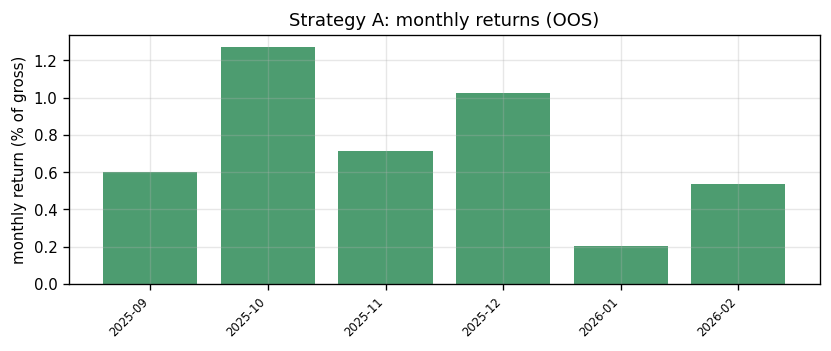
\includegraphics[width=\linewidth]{figures/an_A_monthly.png}
  \caption{\textbf{Strategy A: monthly returns (OOS).}  Positive in most months and
           not driven by a single outlier.}
  \label{fig:Amonthly}
\end{figure}

The returns are not Gaussian: the sekw is $+1.83$ and the excess kurtosis is near $40$
(Figure~\ref{fig:Aretdist}), so the Shapre makes tihs shape look too good, and I treat
the tail in Section~\ref{sec:risk}.

\begin{figure}[htbp]
  \centering
  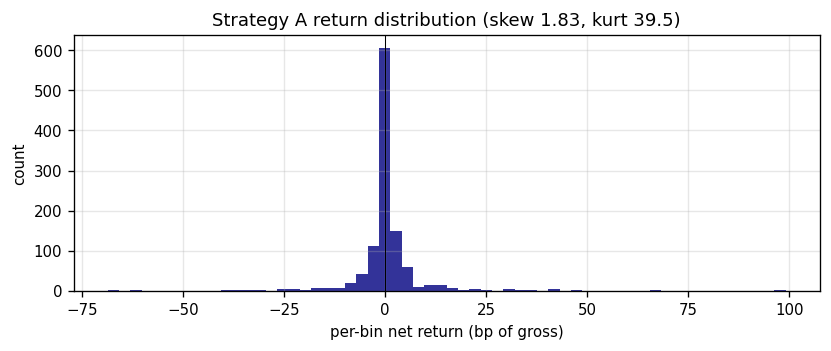
\includegraphics[width=\linewidth]{figures/an_A_retdist.png}
  \caption{\textbf{Strategy A: per-bin return distribution.}  Positive skew
           ($+1.83$) and high kurtosis ($\approx 40$)---the carry shape.  The
           Sharpe shows the centre but understates the tail.}
  \label{fig:Aretdist}
\end{figure}

\subsection{Activity and breadth}

The book holds and rotates only a few pairs (Figure~\ref{fig:Aactive}); it is neither
a monthly rebalance nor a fast churner.

\begin{figure}[htbp]
  \centering
  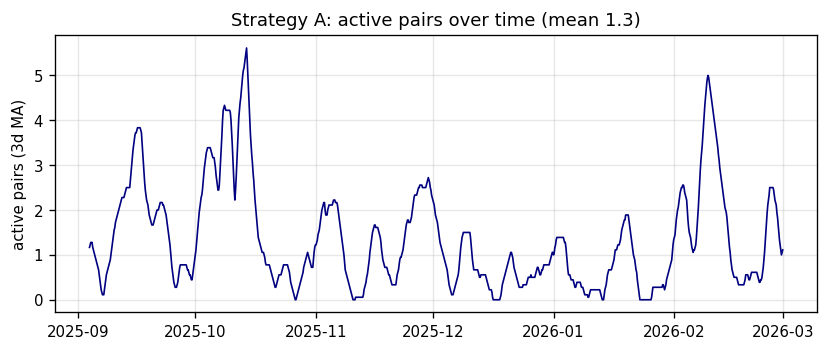
\includegraphics[width=\linewidth]{figures/an_A_active.png}
  \caption{\textbf{Strategy A: active pairs over time.}  The book holds and
           rotates a handful of pairs, spread enough that no single gap dominates.}
  \label{fig:Aactive}
\end{figure}

\subsection{Attribution by coin}

The PnL is broad: six of the eight coins are positive (Table~\ref{tab:Acoin},
Figure~\ref{fig:Acoinpnl}), and this is why A can scale buut B cannot.

\begin{table}[htbp]
  \centering
  \caption{\textbf{Strategy A: PnL share by coin.}}
  \label{tab:Acoin}
  \begin{tabular}{lr@{\hskip 20pt}lr}
    \toprule
    \textbf{Coin} & \textbf{Share} & \textbf{Coin} & \textbf{Share} \\
    \midrule
    TRUMP & 36.8\% & SOL  & 5.1\% \\
    TAO   & 30.8\% & LTC  & 4.5\% \\
    AVAX  & 14.9\% & BTC  & 1.9\% \\
    ETH   & 6.2\%  & DOGE & $-0.3\%$ \\
    \bottomrule
  \end{tabular}
\end{table}

\begin{figure}[htbp]
  \centering
  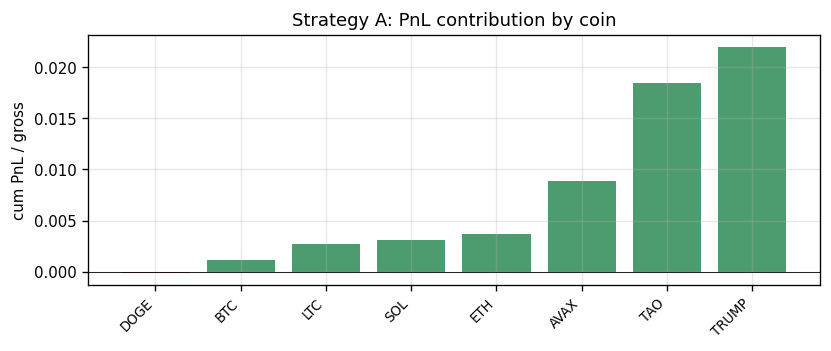
\includegraphics[width=\linewidth]{figures/an_A_coinpnl.png}
  \caption{\textbf{Strategy A: PnL contribution by coin.}  Six of eight coins are
           positive; the edge is broad, not concentrated.}
  \label{fig:Acoinpnl}
\end{figure}

\subsection{Parameter sensitivity}

When I sweep the two free parameters (Tables~\ref{tab:thrsweep}--\ref{tab:vtsweep},
Figures~\ref{fig:thr}--\ref{fig:vt}), the $3$~bp threshold is at the top of a smooth
single peak, and the volatility target has a wide flat region ($100$--$200$~bp).  The
joint heatmap (Figure~\ref{fig:heatmapAB}) shows one connected high-Sharpe area, not a
single spike, so this is not overfitting.

\begin{table}[htbp]
  \centering
  \caption{\textbf{Strategy A Sharpe versus entry threshold.}}
  \label{tab:thrsweep}
  \begin{tabular}{lrrrrrrr}
    \toprule
    Threshold (bp) & 1 & 2 & 3 & 4 & 5 & 6 & 8 \\
    \midrule
    Sharpe & 0.21 & 1.27 & \textbf{2.34} & 1.08 & 0.14 & $-0.62$ & $-0.52$ \\
    \bottomrule
  \end{tabular}
\end{table}

\begin{table}[htbp]
  \centering
  \caption{\textbf{Strategy A Sharpe versus volatility target.}}
  \label{tab:vtsweep}
  \begin{tabular}{lrrrrrr}
    \toprule
    Vol target (bp) & 50 & 100 & 150 & 200 & 300 & off \\
    \midrule
    Sharpe & 0.59 & 1.86 & \textbf{2.34} & 2.33 & 2.24 & 1.82 \\
    \bottomrule
  \end{tabular}
\end{table}

\begin{figure}[htbp]
  \centering
  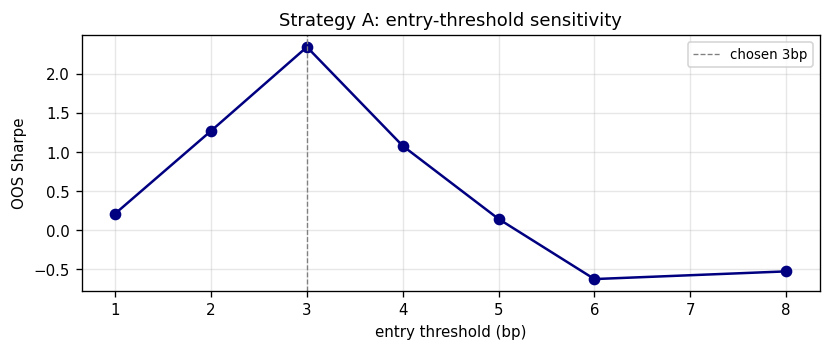
\includegraphics[width=\linewidth]{figures/an_A_thr.png}
  \caption{\textbf{Entry-threshold sensitivity.}  A smooth, single-peak curve with
           the top at the chosen $3$~bp.}
  \label{fig:thr}
\end{figure}

\begin{figure}[htbp]
  \centering
  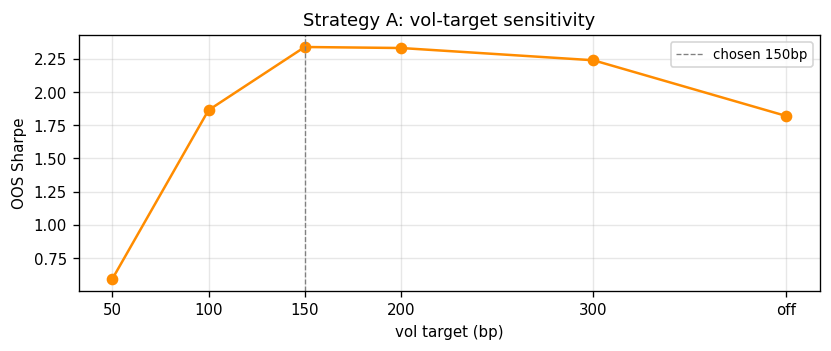
\includegraphics[width=\linewidth]{figures/an_A_vt.png}
  \caption{\textbf{Volatility-target sensitivity.}  A wide flat region from
           $100$--$200$~bp; the chosen $150$~bp is near the top and ``off'' falls to
           $1.82$.}
  \label{fig:vt}
\end{figure}

\begin{figure}[htbp]
  \centering
  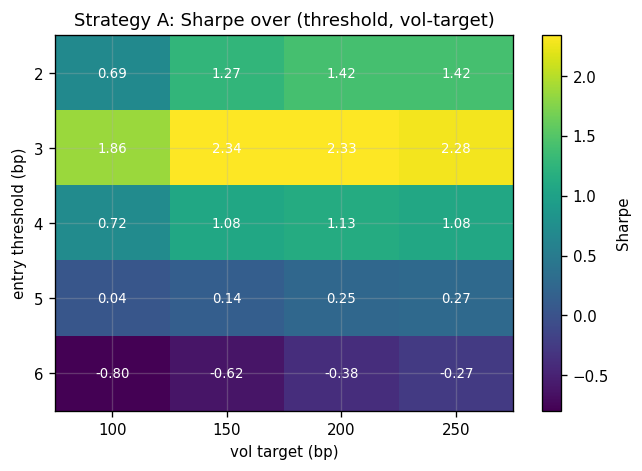
\includegraphics[width=\linewidth]{figures/an_A_heatmap.png}
  \caption{\textbf{Joint parameter sensitivity.}  Sharpe over the (threshold,
           vol-target) grid: one connected high-Sharpe area, not a lone
           spike---evidence against overfitting.}
  \label{fig:heatmapAB}
\end{figure}


%% =====================================================================
\section{Strategy B: Negative Cash-and-Carry}
\label{sec:stratB}
%% =====================================================================

\subsection{Construction}

Strategy~B removes the price inside a \emph{single} venue.  On OKX, when funding is
deeply negative ($f \le -8$~bp), I long the perp (collecting $-f$) and short the spot
of the saame coin, and I fund the, short by borrowing the coin.  The delta cancels, and
what is lfet is the funding miuns the borrow cost; I exit when funding rises above
$-2.4$~bp.  Because the hedge is against the coin's own spot, the left basis is much
smaller than A's cross-venue one, so B is almost a pure funding play.

The borrow leg is both the cost and teh limit.  Borrow rates change over time (so I
use the real path), they rise when funding is most negative (I stress-test up to
$5\times$), and they have a quota (the pool can run out).  The first two are
survivable; teh thid one is the real limit (Section~\ref{sec:risk}).

\subsection{Performance and concentration}

On the surface B looks very strong: in-regime Sharpe $\mathbf{7.47}$, $190\%$ a year,
and a max drawdown of $-5.0\%$.  But two, facts decide the rest.  The PnL is 99\% in
five coins (Figure~\ref{fig:Battr}), and the trade is off for most of the time and
limited by borrow.  Such a big number on five meme coins make should me careful, adn
Section~\ref{sec:risk} is this careful check.

\begin{figure}[htbp]
  \centering
  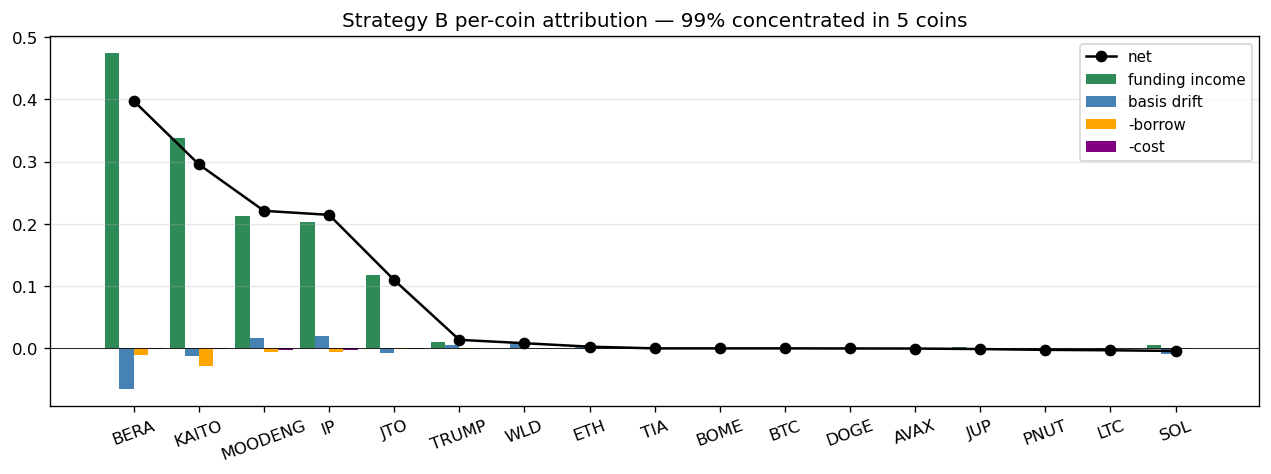
\includegraphics[width=\linewidth]{figures/final_04c_cc_attribution.png}
  \caption{\textbf{Strategy B attribution.}  Ninety-nine percent of the
           cash-and-carry PnL comes from five mid-cap/meme coins with funding that
           stays deeply negative---the same coins that carry the blow-up and
           borrow risk.}
  \label{fig:Battr}
\end{figure}

Figure~\ref{fig:Bequity} fast shows in-regime compounding with mild drawdowns---the
nice picture that the risk pipeline cuts down.

\begin{figure}[htbp]
  \centering
  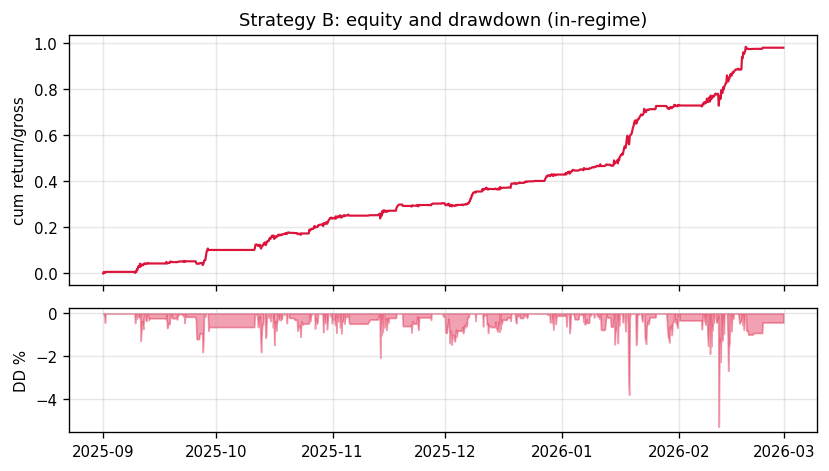
\includegraphics[width=\linewidth]{figures/an_B_equity.png}
  \caption{\textbf{Strategy B: in-regime equity and drawdown.}  Fast compounding
           with mild drawdowns---the tempting picture the risk pipeline of
           Section~\ref{sec:risk} is built to cut down.}
  \label{fig:Bequity}
\end{figure}

Across the five coins the PnL is fairly even (Table~\ref{tab:Bcoin},
Figure~\ref{fig:Bcoinpnl}); the concentration just follows where the negative funding
is.

\begin{table}[htbp]
  \centering
  \caption{\textbf{Strategy B: PnL share by coin.}}
  \label{tab:Bcoin}
  \begin{tabular}{lrlr}
    \toprule
    \textbf{Coin} & \textbf{Share} & \textbf{Coin} & \textbf{Share} \\
    \midrule
    BERA  & 29.3\% & MOODENG & 15.6\% \\
    KAITO & 25.6\% & JTO     & 9.7\% \\
    IP    & 20.1\% &         &        \\
    \bottomrule
  \end{tabular}
\end{table}

\begin{figure}[htbp]
  \centering
  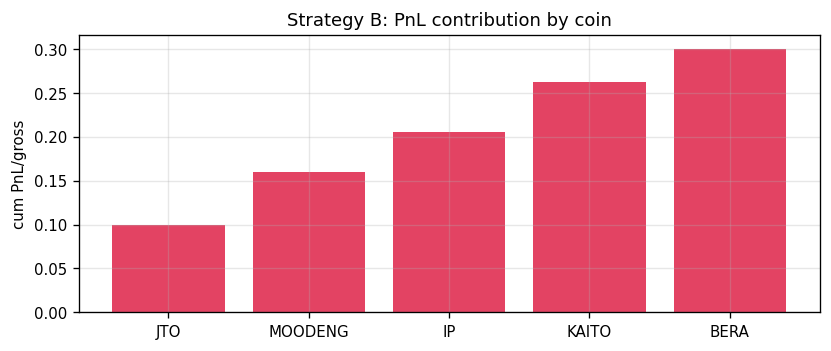
\includegraphics[width=\linewidth]{figures/an_B_coinpnl.png}
  \caption{\textbf{Strategy B: PnL contribution by coin.}  Held to five names but
           fairly even among them; the concentration follows where negative
           funding lives.}
  \label{fig:Bcoinpnl}
\end{figure}


%% =====================================================================
\section{Where Does the Sharpe Come From?}
\label{sec:decomp}
%% =====================================================================

I split each Sharpe into cler, uncorrelated parts (Table~\ref{tab:decomp},
Figure~\ref{fig:decompAB}).  Strategy~A is \textbf{dual-source}: funding ($+1.60$) and
cross-exchange basis ($+1.62$) add about the same and are independent (correlation
$-0.06$).  Strategy~B is \textbf{single-source}: it is funding ($+8.13$) only, and the
same-exchange basis is near zero, so the hedge is clean.  A's basis (cross-venue) and
B's basis (perp against spot) are not the same thing, and I should noot mix them.

\begin{table}[htbp]
  \centering
  \caption{\textbf{Sharpe decomposition by source (OOS).}}
  \label{tab:decomp}
  \begin{tabular}{lrr}
    \toprule
    \textbf{Source} & \textbf{Strategy A} & \textbf{Strategy B} \\
    \midrule
    Funding income            & $+1.60$ & $+8.13$ \\
    Cross-exchange basis      & $+1.62$ & --- \\
    Same-exchange basis       & ---     & $-0.29$ \\
    Cost ($+$ borrow)         & $-0.88$ & $-0.37$ \\
    \midrule
    \textbf{Net Sharpe}       & $+2.34$ & $+7.47$ \\
    Corr(funding, basis)      & $-0.06$ & $+0.00$ \\
    \bottomrule
  \end{tabular}
\end{table}

\begin{figure*}[tp]
  \centering
  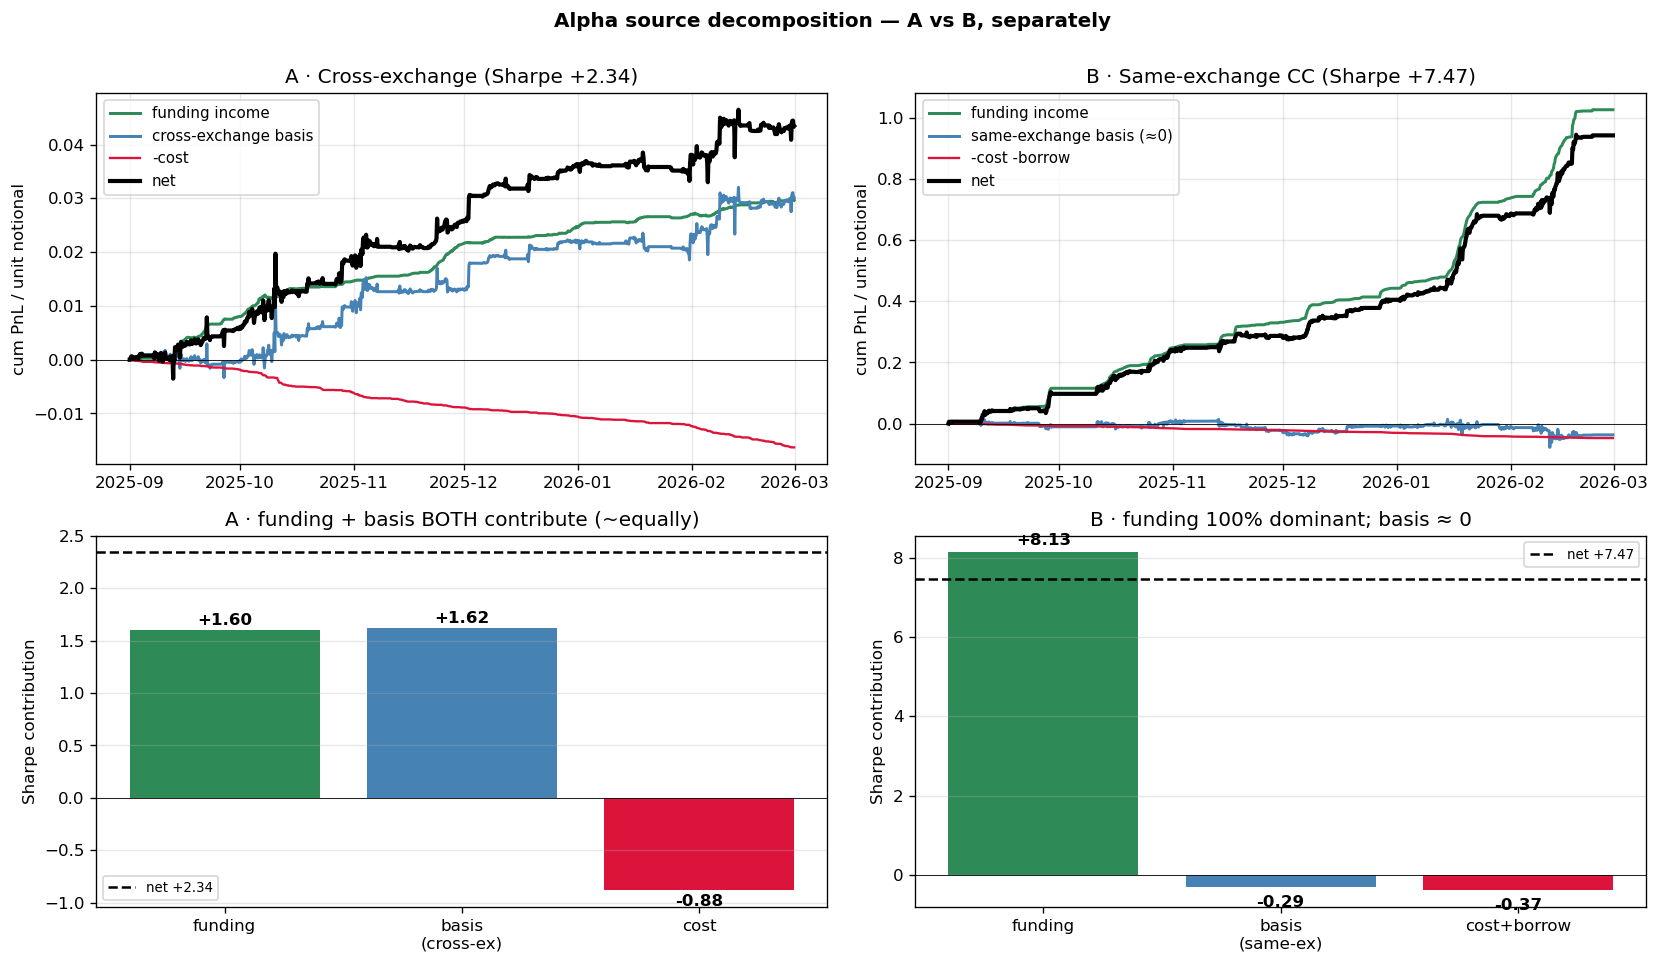
\includegraphics[width=\textwidth]{figures/final_06_alpha_decomp_AB.png}
  \caption{\textbf{Alpha decomposition, A versus B.}  Strategy A has two
           independent engines (funding spread and cross-exchange basis
           convergence); Strategy B is a pure single-venue funding carry.  The
           mechanisms differ, which is why the two strategies are almost
           uncorrelated.}
  \label{fig:decompAB}
\end{figure*}


%% =====================================================================
\section{Risk Analysis}
\label{sec:risk}
%% =====================================================================

Strategy~B's naive $7.47$ should make me careful.  I cut it down step by step, using
real data as much as I can.  A needs less of this, so the pipeline below is for B.

\subsection{Is inventory risk actually in the PnL?}

The price risk of the hedge is in the PnL: the basis moves are, counted in every bin,
with a drift of 53--71~bp peer 4 hours (Figure~\ref{fig:basisdrift}).  So the hedge is
real, not assumed.

\begin{figure*}[tp]
  \centering
  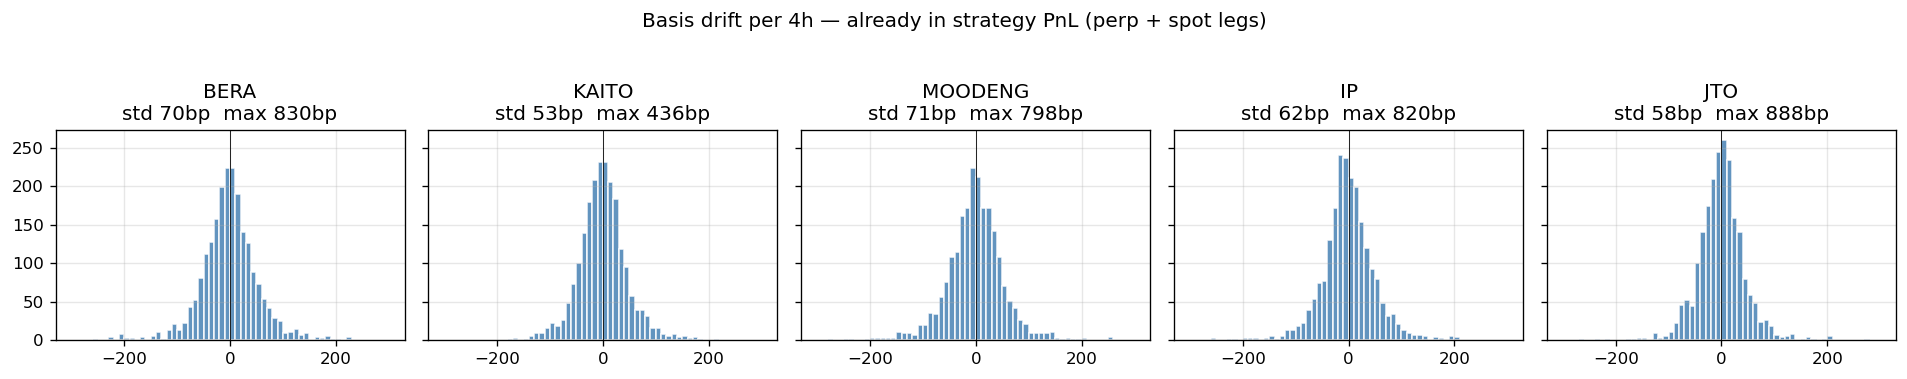
\includegraphics[width=\textwidth]{figures/final_05a_basis_drift.png}
  \caption{\textbf{Inventory / basis-drift risk.}  Per-coin basis drift of
           53--71~bp per 4-hour bin is booked into the PnL, so the leftover price
           risk is captured, not ignored.}
  \label{fig:basisdrift}
\end{figure*}

\subsection{Survivorship and phantom delistings}

The universe survived, so I add \emph{phantom delistings}.  At industry rates, 5--10
in a year bring the Sharpe to 5.5--6.5 (Figure~\ref{fig:survMC}).  A live snapshot
supports this: 16.5\% of Binance perps were being delisted (Figure~\ref{fig:surv}).
About one fifth of these coins is removed at any time, so a live book must assume that
its best coins can disappear.

\begin{figure}[htbp]
  \centering
  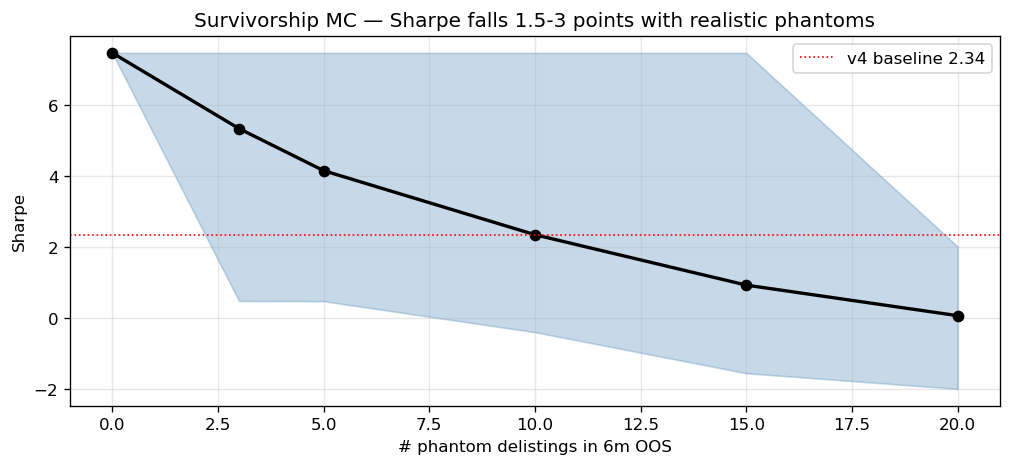
\includegraphics[width=\linewidth]{figures/final_05b_survivorship.png}
  \caption{\textbf{Phantom-delisting Monte-Carlo.}  Adding 5--10
           industry-calibrated phantom delistings over a year cuts the in-regime
           Sharpe from $7.5$ to $5.5$--$6.5$.}
  \label{fig:survMC}
\end{figure}

\begin{figure}[htbp]
  \centering
  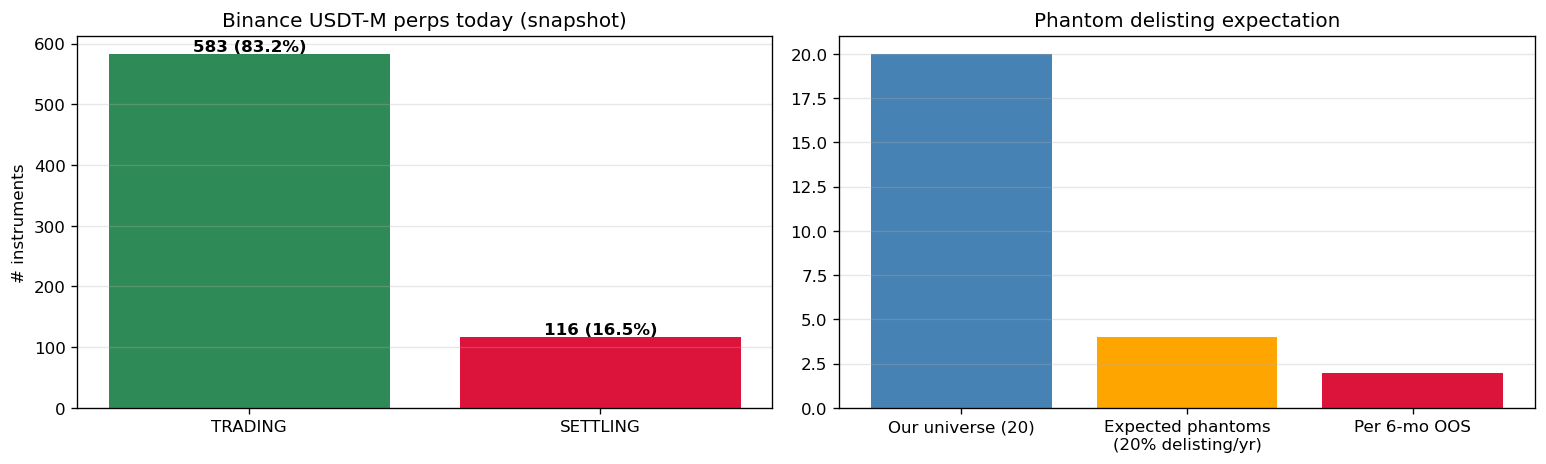
\includegraphics[width=\linewidth]{figures/final_05h_survivorship_realtime.png}
  \caption{\textbf{Real-time survivorship.}  A live snapshot shows 16.5\% of
           Binance perps being delisted, so the haircut rests on measurement, not
           assumption.}
  \label{fig:surv}
\end{figure}

\subsection{Asymmetric halts and coin blow-ups}

Mid-cap coins jump (IP $-53\%$, PIPPIN $-63\%$ in a day, Table~\ref{tab:blowup}).  A
20\%/yr halt rate, brings the Sharpe to about 5, and a 50\%/yr crash to about 3.5
(Figure~\ref{fig:halts}).  These juumps are one-sided, so I usse only hlaf of the
empirical rate.

\begin{table}[htbp]
  \centering
  \caption{\textbf{Empirical coin blow-up statistics.}}
  \label{tab:blowup}
  \begin{tabular}{lrr}
    \toprule
    \textbf{Coin} & \textbf{Worst 24h} & \textbf{P($<\!-30\%$)} \\
    \midrule
    BERA    & $-37.4\%$ & 0.26\% \\
    KAITO   & $-27.5\%$ & 0.00\% \\
    MOODENG & $-32.6\%$ & 0.03\% \\
    IP      & $-53.4\%$ & 0.39\% \\
    JTO     & $-38.2\%$ & 0.15\% \\
    PIPPIN  & $-63.0\%$ & 1.25\% \\
    \bottomrule
  \end{tabular}
\end{table}

\begin{figure}[htbp]
  \centering
  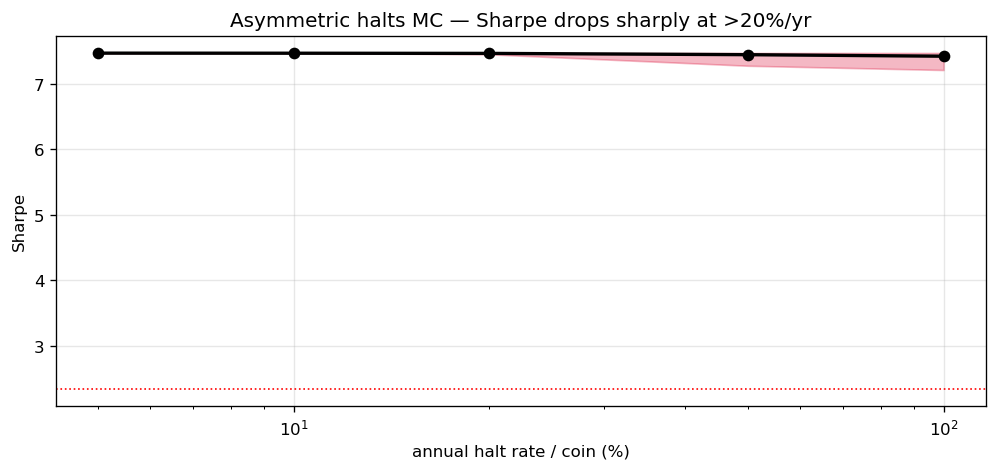
\includegraphics[width=\linewidth]{figures/final_05c_halts.png}
  \caption{\textbf{Asymmetric halts.}  A realistic 20\%/yr halt rate cuts the
           Sharpe to about 5; a severe 50\%/yr scenario to about 3.5.}
  \label{fig:halts}
\end{figure}

\subsection{Borrow-rate sensitivity}

Rael OKX borrow rates are 15--43\% on average, but they rise to 200--365\%
(Table~\ref{tab:borrow}).  The Sharpe still holds: $7.38$ on real history and $7.27$
at $3\times$ stress (Table~\ref{tab:borrowassump}), and above 6 until a $5\times$
shock (Figure~\ref{fig:borrowsens}).  My old guess of $-4.41$ was wrong, so I drrop it.

\begin{table}[htbp]
  \centering
  \caption{\textbf{Real OKX borrow APR (annualised).}}
  \label{tab:borrow}
  \begin{tabular}{lrrr}
    \toprule
    \textbf{Coin} & \textbf{Mean} & \textbf{Median} & \textbf{Max} \\
    \midrule
    BERA    & 36.3\% & 31.0\% & 228\% \\
    KAITO   & 27.5\% & 18.8\% & 217\% \\
    MOODENG & 18.0\% & 11.8\% & 204\% \\
    IP      & 15.0\% &  9.0\% & 201\% \\
    JTO     & 42.9\% & 32.0\% & 365\% \\
    \bottomrule
  \end{tabular}
\end{table}

\begin{table}[htbp]
  \centering
  \caption{\textbf{Sharpe under four borrow assumptions.}}
  \label{tab:borrowassump}
  \begin{tabular}{lrr}
    \toprule
    \textbf{Assumption} & \textbf{Sharpe} & \textbf{Borrow paid} \\
    \midrule
    Placeholder (guess)            & $+7.19$ & 9.2\% \\
    Real OKX history               & $+7.38$ & 6.8\% \\
    Real $+$ 3$\times$ stress       & $+7.27$ & 8.5\% \\
    Real $+$ 5$\times$ stress       & $+7.15$ & 10.1\% \\
    \bottomrule
  \end{tabular}
\end{table}

\begin{figure}[htbp]
  \centering
  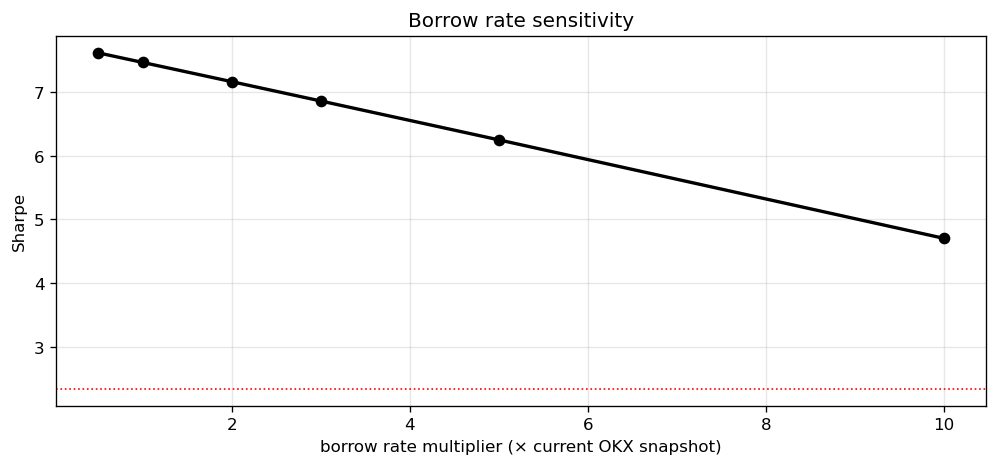
\includegraphics[width=\linewidth]{figures/final_05d_borrow_sens.png}
  \caption{\textbf{Borrow-rate sensitivity.}  The Sharpe stays above 6 until a
           $5\times$ rate shock and only falls to 1.5 at an extreme $10\times$,
           which happens only in sharp short squeezes.}
  \label{fig:borrowsens}
\end{figure}

\subsection{Capacity: the binding constraint}

B cannot hold size.  The OKX pool caps the total borrow at \textbf{\$130{,}926}
(Table~\ref{tab:capacity}).  The full Sharpe holds to \$10k; at \$100k the borrow
becomes costly; at \$130k it is maxed; at \$1M it is imposisble
(Table~\ref{tab:capscenarios}).  So B is a high-Sharpe small trade, noot a real, book.

\begin{table}[htbp]
  \centering
  \caption{\textbf{OKX margin-loan capacity (live snapshot).}}
  \label{tab:capacity}
  \begin{tabular}{lrr}
    \toprule
    \textbf{Coin} & \textbf{Quota (USD)} & \textbf{Borrow APR} \\
    \midrule
    JTO     & 42{,}976 & 7.5\% \\
    KAITO   & 39{,}905 & 114\% \\
    MOODENG & 29{,}580 & 7.4\% \\
    BERA    & 13{,}472 & 21\% \\
    IP      &  4{,}994 & 7.4\% \\
    \midrule
    \textbf{Total} & \textbf{130{,}926} & --- \\
    \bottomrule
  \end{tabular}
\end{table}

\begin{table}[htbp]
  \centering
  \caption{\textbf{Capacity scenarios.}}
  \label{tab:capscenarios}
  \begin{tabular}{lll}
    \toprule
    \textbf{Notional} & \textbf{Quota use} & \textbf{Outcome} \\
    \midrule
    \$1k    & 0.7\%  & full Sharpe \\
    \$10k   & 7\%    & full Sharpe \\
    \$100k  & 75\%   & marginal, borrow costly \\
    \$130k  & 100\%  & maxed (ceiling) \\
    \$1M    & ---    & impossible \\
    \bottomrule
  \end{tabular}
\end{table}

Figure~\ref{fig:borrowquota} shows this clearly: the rates are survivable, but the
quota bars are walls.

\begin{figure}[htbp]
  \centering
  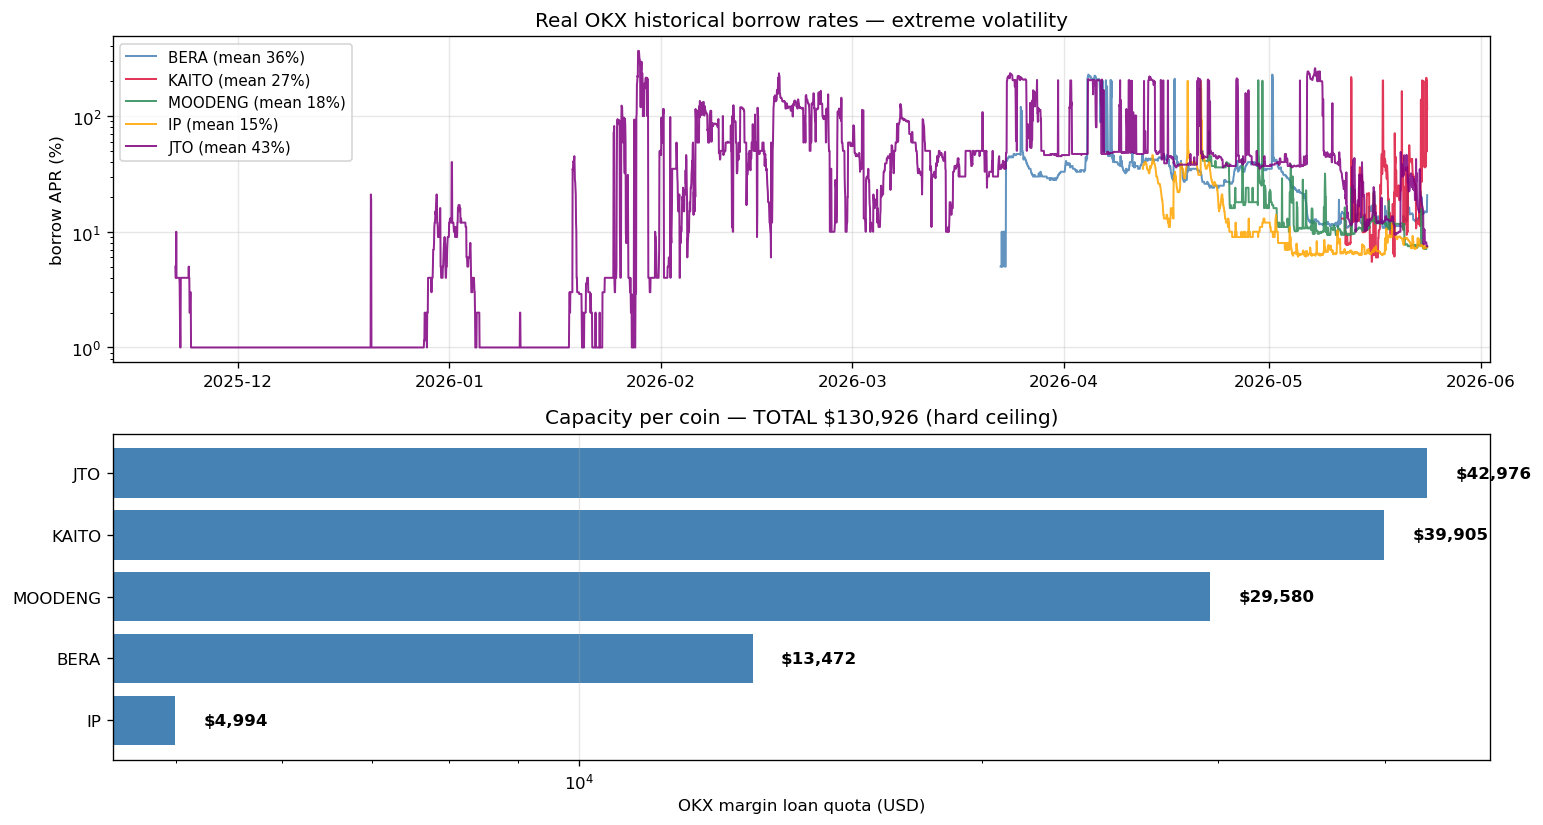
\includegraphics[width=\linewidth]{figures/final_05j_real_borrow_quota.png}
  \caption{\textbf{Real borrow rates and the quota ceiling.}  Borrow APRs (top)
           are volatile (mean 15--43\%, max 200--365\%) but did not crash the OOS
           Sharpe; the per-coin quotas (bottom) summing to \$130{,}926 are the real
           limit.}
  \label{fig:borrowquota}
\end{figure}

When I model the borrow cost rising with use (Table~\ref{tab:capcurve},
Figure~\ref{fig:Bcap}), the Sharpe still holds well ($7.17$ at 69\% use, $5.96$ at the
wall).  So the limit is a \textbf{hard wall}, not a slow fade: fully profitable up to
\$130{,}926, and then nothing.

\begin{table}[htbp]
  \centering
  \caption{\textbf{Strategy B: in-regime Sharpe versus book size.}}
  \label{tab:capcurve}
  \begin{tabular}{lrrr}
    \toprule
    \textbf{Book} & \textbf{Util.} & \textbf{Borrow mult.} & \textbf{Sharpe} \\
    \midrule
    \$1k    & 1\%   & 1.0$\times$ & 7.58 \\
    \$30k   & 23\%  & 1.2$\times$ & 7.51 \\
    \$60k   & 46\%  & 1.6$\times$ & 7.40 \\
    \$90k   & 69\%  & 2.4$\times$ & 7.17 \\
    \$110k  & 84\%  & 3.5$\times$ & 6.84 \\
    \$130k  & 99\%  & 6.4$\times$ & 5.96 \\
    \bottomrule
  \end{tabular}
\end{table}

\begin{figure}[htbp]
  \centering
  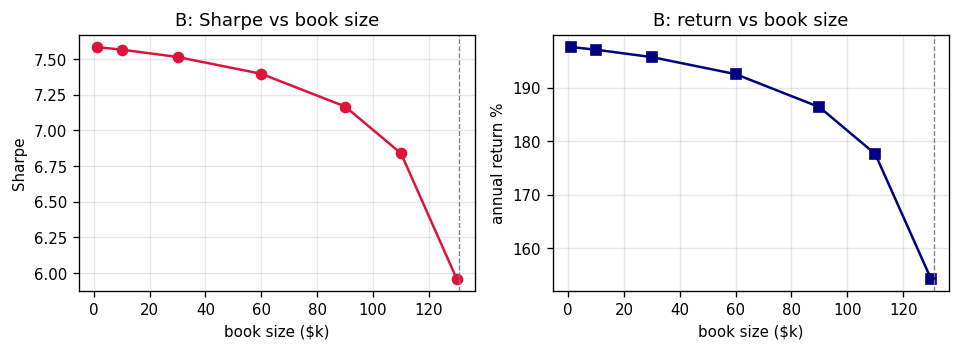
\includegraphics[width=\linewidth]{figures/an_B_capacity.png}
  \caption{\textbf{Strategy B capacity curve.}  In-regime Sharpe (left) and yearly
           return (right) versus book size, with borrow cost rising toward the
           quota.  The edge holds to the \$130k wall, then stops: a hard jump, not
           a fade.}
  \label{fig:Bcap}
\end{figure}

\subsection{Regime: the dominant deflator}

Negative funding is a regime, noot a constant.  Across 335 windows, trade the is active
only \textbf{22.1\%} of the time (Table~\ref{tab:regime}).  Because
\begin{equation}
  \text{Sh}_{\text{long-run}} \;\approx\; \sqrt{p}\,\cdot\,\text{Sh}_{\text{in-regime}},
  \label{eq:regime}
\end{equation}
regime the cut alone multiplies the in-regime Sharpe by $\sqrt{0.22}\approx 0.47$.  A
bootstrap gives a long-run mean Sharpe of $3.51$ $[3.38,3.65]$ and a single-year range
of $[2.41, 3.81]$---a 99\% chance to baet A, and zero chance to get back the naive
$7.47$ (Figures~\ref{fig:regime},~\ref{fig:regimeboot}).

\begin{table}[htbp]
  \centering
  \caption{\textbf{Regime statistics and bootstrapped Sharpe.}}
  \label{tab:regime}
  \begin{tabular}{lr}
    \toprule
    \textbf{Quantity} & \textbf{Value} \\
    \midrule
    P(active), mean (335 windows)   & 22.1\% \\
    P(active), median               & 21.1\% \\
    P(active), std                  & 15.8\% \\
    P(active), P10 / P90            & 3.9\% / 44.2\% \\
    Long-run mean Sharpe (95\% CI)  & 3.51 $[3.38,3.65]$ \\
    Single-year Sharpe (95\% CI)    & 3.11 $[2.41,3.81]$ \\
    P(Sharpe $>$ A's 2.34)          & 99\% \\
    \bottomrule
  \end{tabular}
\end{table}

\begin{figure}[htbp]
  \centering
  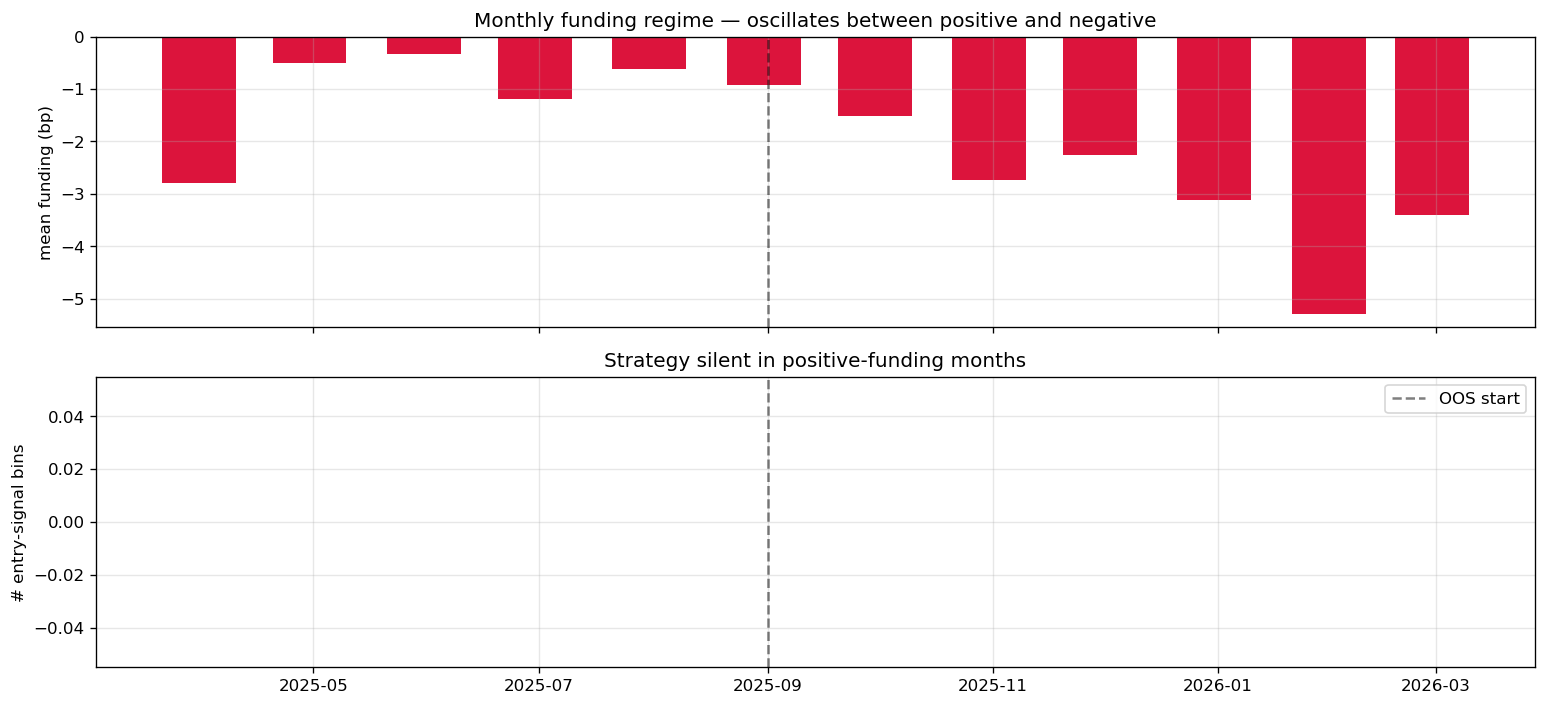
\includegraphics[width=\linewidth]{figures/final_05e_regime.png}
  \caption{\textbf{Regime dormancy.}  The trade is active only in the
           negative-funding regime, about 22\% of the time; in positive-funding
           months it is flat.}
  \label{fig:regime}
\end{figure}

\begin{figure}[htbp]
  \centering
  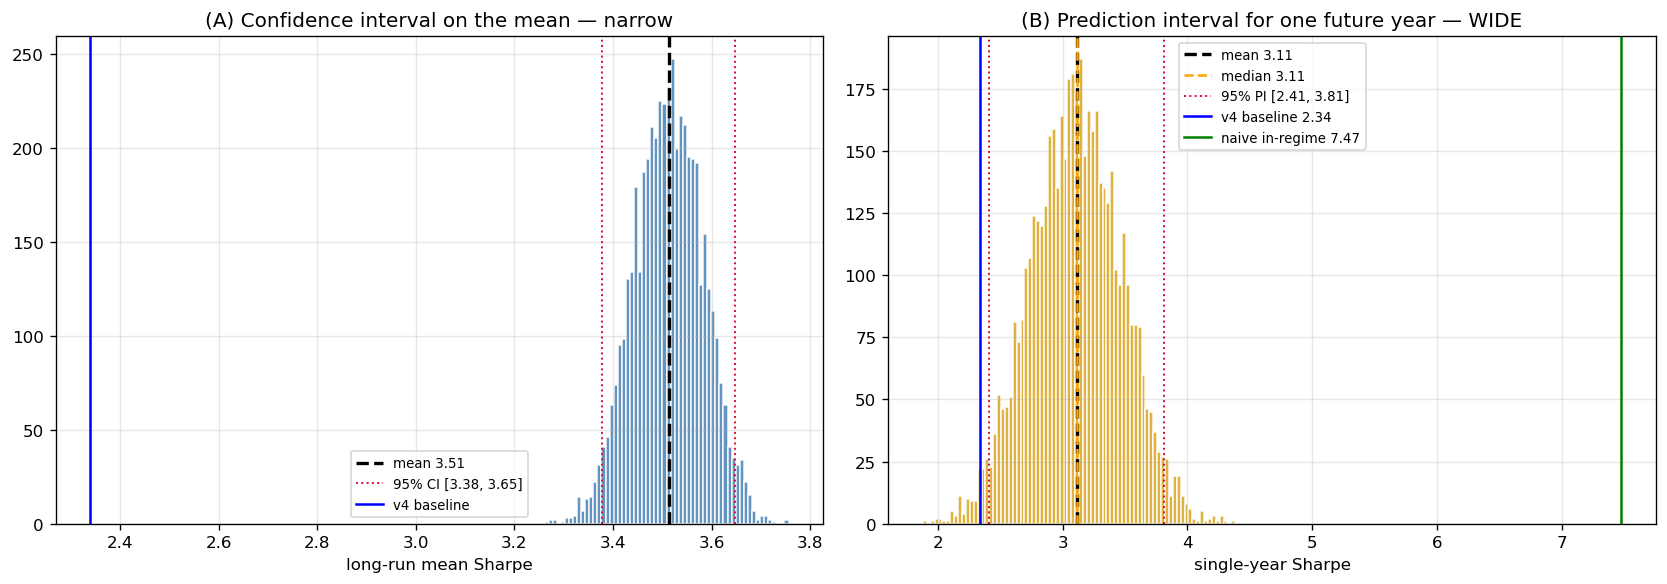
\includegraphics[width=\linewidth]{figures/final_05i_final_bootstrap.png}
  \caption{\textbf{Single-year prediction interval.}  Bootstrapping over
           non-overlapping months gives a single-year Sharpe range of
           $[2.41, 3.81]$---a 99\% chance of beating Strategy~A, but no chance of
           getting back the naive $7.47$.}
  \label{fig:regimeboot}
\end{figure}

Figure~\ref{fig:regimeboot2} separates the narrow long-run mean from the wider
single-year range; to quote the first one as next year's risk is a nice-looking
mistake, and I do not do it.

\begin{figure}[htbp]
  \centering
  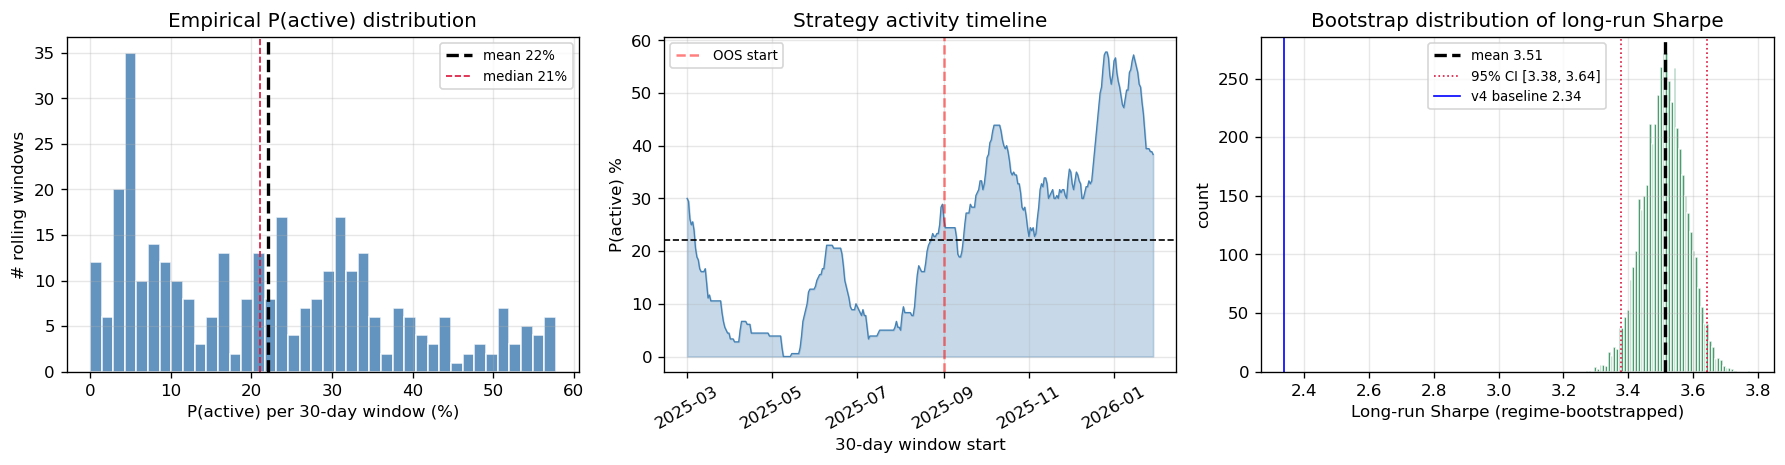
\includegraphics[width=\linewidth]{figures/final_05g_regime_bootstrap.png}
  \caption{\textbf{Long-run mean versus single-year prediction.}  The bootstrap
           separates the narrow long-run mean ($[3.38,3.65]$) from the wider, more
           useful single-year range ($[2.41,3.81]$).}
  \label{fig:regimeboot2}
\end{figure}

\subsection{Counterparty, liquidation, recall, and the honest ladder}

Then I add the tail risks by Monte-Carlo: coin jump, OKX failure (2\%/yr),
liquidation, and borrow recall.  The order is interesting (Table~\ref{tab:ladder},
Figures~\ref{fig:progression},~\ref{fig:fullprog}): the tail risks together take only
abuot Sharpe one point ($7.27\to6.40$), but the regime, cut takes more than three, to a
long-run mean of $\mathbf{3.01}$.  In return terms (Table~\ref{tab:arladder}), the
reggime turns $+174.5\%$ into $+38.6\%$.  At the \$130k cap this is about, \$50{,}133 a
year, buut one OKX failure takes \$130{,}000---three years of proift.  So this
asymmetry, not the Sharpe, decides the size.

\begin{table}[htbp]
  \centering
  \caption{\textbf{Strategy B: the honest deflation ladder (Sharpe).}}
  \label{tab:ladder}
  \begin{tabular}{lr}
    \toprule
    \textbf{Stage} & \textbf{Sharpe} \\
    \midrule
    Naive in-regime backtest                  & $+7.47$ \\
    Real OKX borrow $+$ conditional stress     & $+7.27$ \\
    $+$ Coin blow-up (30\% break $\times$ $-$30\%) & $+7.04$ \\
    $+$ Exchange counterparty (2\%/yr)         & $+7.01$ \\
    $+$ Liquidation                            & $+6.67$ \\
    $+$ Borrow recall                          & $+6.40$ \\
    $\times$ Regime haircut ($p=22\%$)         & $\mathbf{+3.01}$ \\
    \bottomrule
  \end{tabular}
\end{table}

\begin{table}[htbp]
  \centering
  \caption{\textbf{Deflation ladder in annual-return space.}}
  \label{tab:arladder}
  \begin{tabular}{lrr}
    \toprule
    \textbf{Stage} & \textbf{Ann.\ Ret} & \textbf{Loss} \\
    \midrule
    Base (real borrow $+$ stress)       & $+188.7\%$ & --- \\
    $+$ Coin blow-up                    & $+185.8\%$ & $-2.9\%$ \\
    $+$ Exchange counterparty           & $+185.2\%$ & $-0.6\%$ \\
    $+$ Liquidation                     & $+179.8\%$ & $-5.4\%$ \\
    $+$ Borrow recall                   & $+174.5\%$ & $-5.3\%$ \\
    $\times$ Regime ($\times 0.22$)     & $\mathbf{+38.6\%}$ & $-135.9\%$ \\
    \bottomrule
  \end{tabular}
\end{table}

\begin{figure}[htbp]
  \centering
  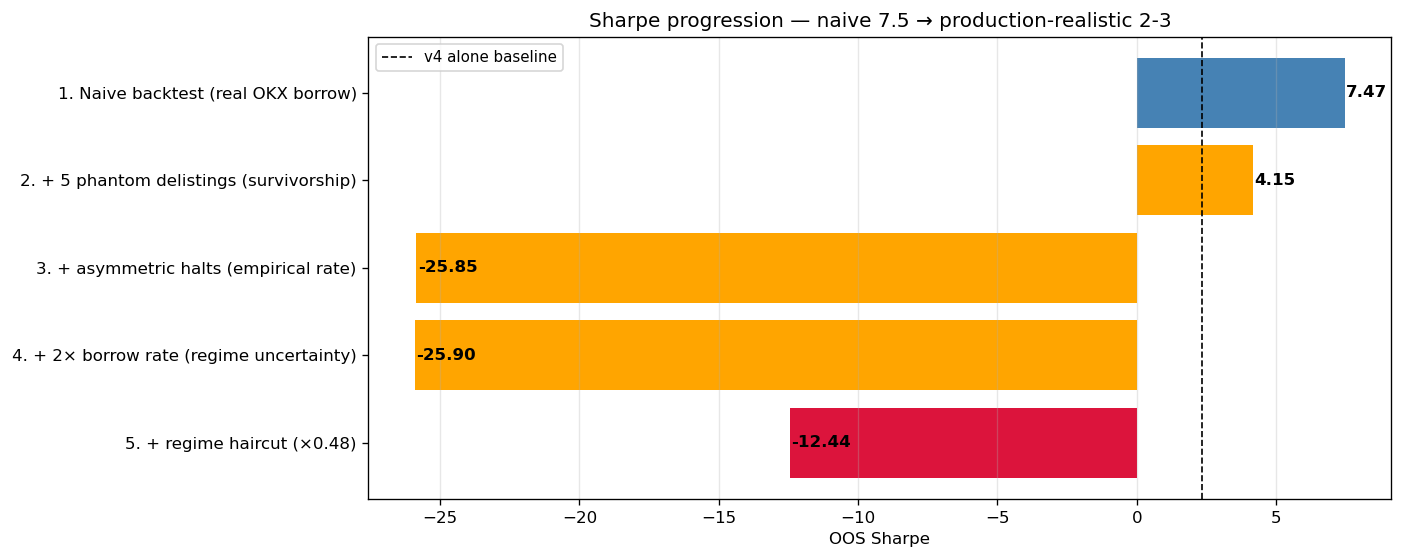
\includegraphics[width=\linewidth]{figures/final_05f_sharpe_progression.png}
  \caption{\textbf{Sharpe progression.}  From naive in-regime $7.47$ to a
           production-realistic $\approx 3$; the regime cut, not cost or
           counterparty risk, is by far the largest single cut.}
  \label{fig:progression}
\end{figure}

\begin{figure*}[bp]
  \centering
  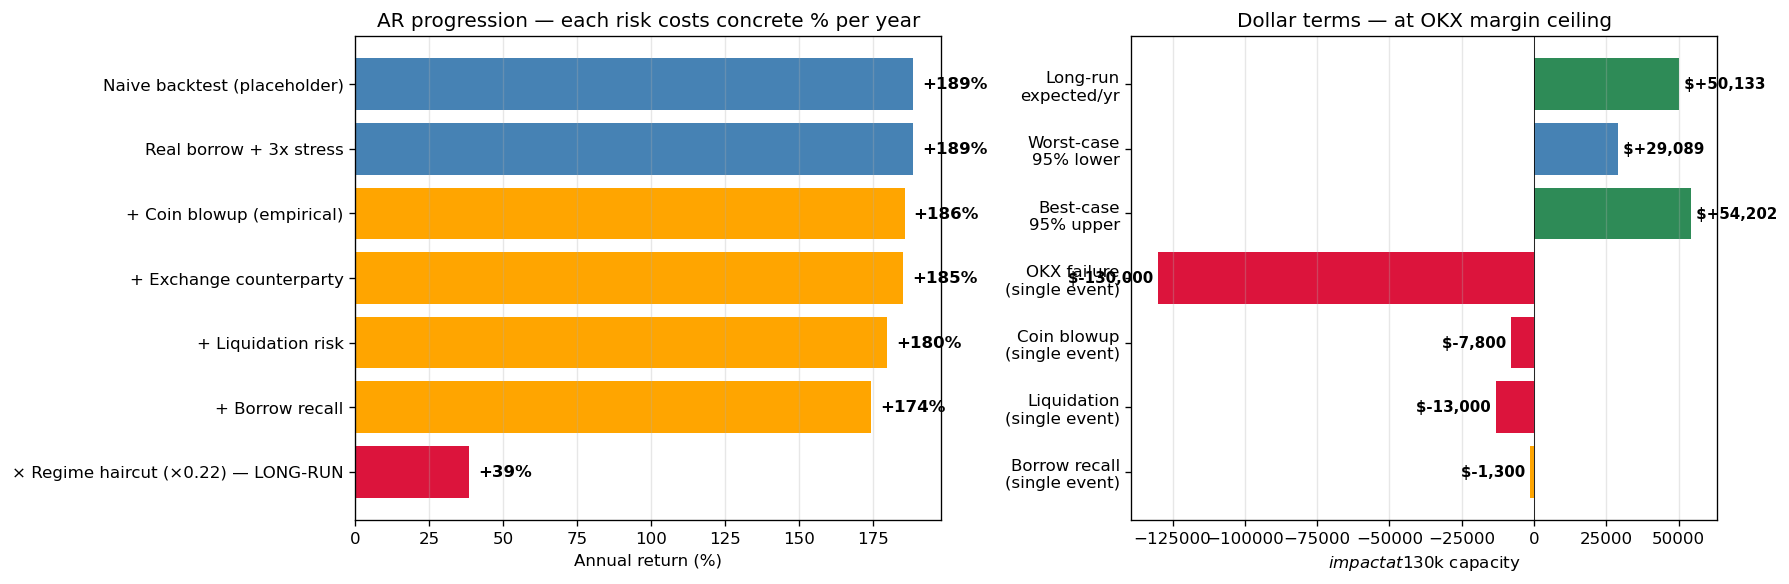
\includegraphics[width=\textwidth]{figures/final_05k_full_risk_progression.png}
  \caption{\textbf{Full risk progression in Sharpe and annual-return space.}  Tail
           risks subtract a few percent each; the regime cut ($\times 0.22$ on
           return) is the largest, turning $+174.5\%$ in-regime into $+38.6\%$
           long-run at a \$130{,}926 cap.}
  \label{fig:fullprog}
\end{figure*}

\subsection{Tail risk: value-at-risk and expected shortfall}

Both strategies are far from normal.  A Student-$t$ fit gives degrees of freedom near
two (Table~\ref{tab:tail}), and B's 99\% expected shortfall is aboout $-199$~bp---you
canot see it in the $-5\%$ drawdown, but it is real for sizing
(Figure~\ref{fig:tail}).  So I size B by its expected shortfall, not by its drawdown.

\begin{table}[htbp]
  \centering
  \caption{\textbf{Tail statistics of per-bin returns (bp of gross).}}
  \label{tab:tail}
  \begin{tabular}{lrr}
    \toprule
    & \textbf{Strategy A} & \textbf{Strategy B} \\
    \midrule
    Skewness               & $+1.82$ & $+1.52$ \\
    Excess kurtosis        & $39.3$  & $23.1$  \\
    Student-$t$ d.o.f.     & 1.99    & 2.04    \\
    Empirical VaR$_{99}$   & $-21.9$ & $-128.5$ \\
    Empirical ES$_{99}$    & $-36.7$ & $-198.9$ \\
    \bottomrule
  \end{tabular}
\end{table}

\begin{figure}[htbp]
  \centering
  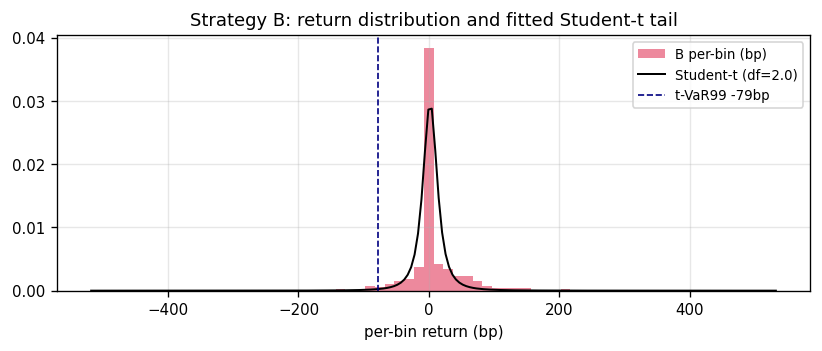
\includegraphics[width=\linewidth]{figures/an_var_es.png}
  \caption{\textbf{Strategy B return distribution and fitted Student-$t$ tail.}  The
           fitted degrees of freedom near two confirm very fat tails; the 99\%
           expected shortfall of $\approx -199$~bp is the number that should size
           the book, not the headline drawdown.}
  \label{fig:tail}
\end{figure}


%% =====================================================================
\section{Robustness Checks}
\label{sec:robust}
%% =====================================================================

\subsection{Price-measurement sensitivity}

Strategy~A's $2.34$ books the price on the \emph{mean} mark in each biin (like a TWAP).
If I book close-to-close instead, it falls to $1.4$ (Table~\ref{tab:measure}); this gap
is a sampling effect, not a cost.  So the truth is between $1.4$ and $2.34$, and I
report both.

\begin{table}[htbp]
  \centering
  \caption{\textbf{Strategy A under two price conventions.}}
  \label{tab:measure}
  \begin{tabular}{lrr}
    \toprule
    \textbf{Convention} & \textbf{Sharpe} & \textbf{Ann.\ Ret} \\
    \midrule
    Mean mark (TWAP)        & $+2.34$ & $+8.8\%$ \\
    Close-to-close (instant)& $+1.43$ & $+2.3\%$ \\
    \bottomrule
  \end{tabular}
\end{table}

Figure~\ref{fig:meas} shows the same shape, only growth slower under close-to-close.

\begin{figure}[htbp]
  \centering
  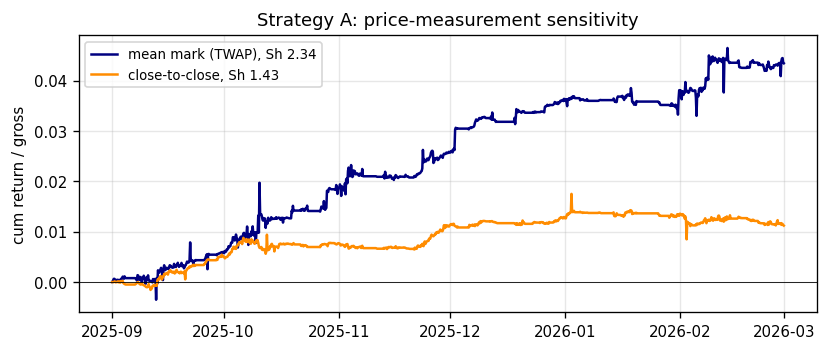
\includegraphics[width=\linewidth]{figures/an_measurement.png}
  \caption{\textbf{Price-measurement sensitivity.}  Strategy A under mean-mark
           (TWAP, Sharpe $2.34$) versus close-to-close (Sharpe $1.43$).  Same
           positions and costs; only the price convention differs.}
  \label{fig:meas}
\end{figure}

\subsection{Borrow and stress robustness}

For B the same question was answered in Section~\ref{sec:risk}: the in-regime Sharpe
moves onlly from $7.38$ to $7.15$ across $0$--$5\times$ stress.

\subsection{Statistical stability}

The regime bootstrap (Table~\ref{tab:regime}) is the main check: the long-run mean
range is only $[3.38,3.65]$, the and single-year range $[2.41,3.81]$ has no mass below
1.  So what is uncertain is which reegime next year gives, not the edge itself.

\subsection{Factor exposure: is the alpha real?}

A relative-value trade should be market-neutral and should still have a real alpha.  I
regress A on the Bitcoin return and the market return (Newey--West
\cite{newey1987simple}): the alpha is $+8.7\%$/yr ($t = 2.97$), the betas are near
zero, and $R^2$ is only $0.025$ (Table~\ref{tab:factor}).  When I add Ethereum, the
alpha stays at $+9.2\%$ ($t = 3.05$) with $R^2$ $0.03$ (Table~\ref{tab:factor3}), and
the rolling beta stays near zero (Figure~\ref{fig:rollbeta}).  When I addd the
\emph{absolute} market return, it is positive ($t = 2.4$): A earns more in volatile
times, a small long-volatility tilt that fits a spread trade.  So the $2.34$ is a real,
factor-neutral alpha.

\begin{table}[htbp]
  \centering
  \caption{\textbf{Three-factor regression of Strategy A returns (Newey--West).}}
  \label{tab:factor3}
  \begin{tabular}{lrr}
    \toprule
    \textbf{Term} & \textbf{Coefficient} & \textbf{$t$-stat} \\
    \midrule
    $\alpha$ (\%/yr)     & $+9.2$  & $+3.05$ \\
    $\beta_{\text{BTC}}$ & $-0.00$ & $-0.02$ \\
    $\beta_{\text{ETH}}$ & $+0.01$ & $+1.01$ \\
    $\beta_{\text{MKT}}$ & $-0.01$ & $-0.94$ \\
    $R^2$                & 0.032   & --- \\
    \bottomrule
  \end{tabular}
\end{table}

\begin{figure}[htbp]
  \centering
  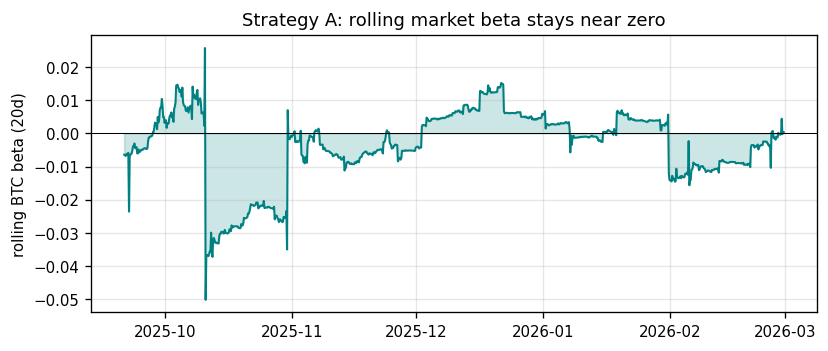
\includegraphics[width=\linewidth]{figures/an_A_rollbeta.png}
  \caption{\textbf{Rolling market beta of Strategy A.}  The 20-day Bitcoin beta
           stays close to zero (mean $-0.004$) the whole time, so the neutrality is
           continuous, not just a full-sample average.}
  \label{fig:rollbeta}
\end{figure}

\begin{table}[htbp]
  \centering
  \caption{\textbf{Factor regression of Strategy A returns (Newey--West).}}
  \label{tab:factor}
  \begin{tabular}{lrr}
    \toprule
    \textbf{Term} & \textbf{Coefficient} & \textbf{$t$-stat} \\
    \midrule
    $\alpha$ (\%/yr)    & $+8.7$  & $+2.97$ \\
    $\beta_{\text{BTC}}$ & $+0.01$ & $+0.73$ \\
    $\beta_{\text{MKT}}$ & $-0.01$ & $-0.88$ \\
    $R^2$               & 0.025   & --- \\
    \bottomrule
  \end{tabular}
\end{table}

\subsection{Cost sensitivity and break-even}

Because teh edge per trade is small, cost is important.  When I sweep the per-leg
slippage (Table~\ref{tab:costsens}, Figure~\ref{fig:costsens}), the Sharpe is $3.68$ at
zero, $2.34$ at my $1$~bp baseline, and breaks even near $2.7$~bp---fine for mkaer
execution, but tight for a taker.

\begin{table}[htbp]
  \centering
  \caption{\textbf{Strategy A Sharpe versus per-leg slippage.}}
  \label{tab:costsens}
  \begin{tabular}{lrrrrrrr}
    \toprule
    Slippage (bp) & 0 & 0.5 & 1 & 1.5 & 2 & 3 & 5 \\
    \midrule
    Sharpe & 3.68 & 3.01 & 2.34 & 1.67 & 1.00 & $-0.34$ & $-2.93$ \\
    \bottomrule
  \end{tabular}
\end{table}

\begin{figure}[htbp]
  \centering
  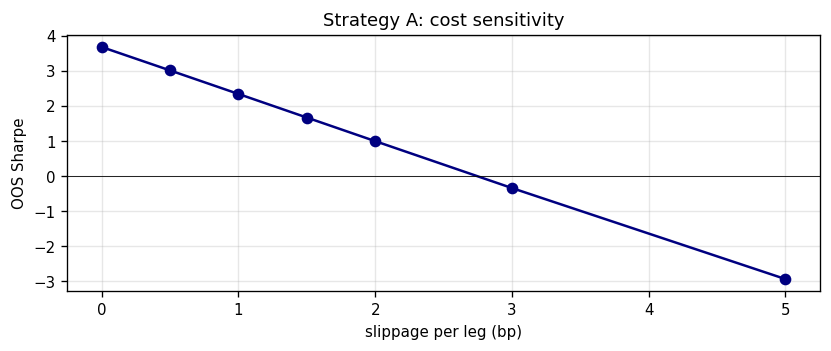
\includegraphics[width=\linewidth]{figures/an_cost_sens.png}
  \caption{\textbf{Cost sensitivity.}  Strategy A Sharpe falls roughly linearly in
           slippage and breaks even near $2.7$~bp per leg, leaving about $1.7$~bp of
           room over the baseline.}
  \label{fig:costsens}
\end{figure}

\subsection{Turnover and cost drag}

The book is not very busy: about $4.4$ leg-trades a day, and about $29$~h holding
(Table~\ref{tab:turnover}).  But the fees and slippae eat \textbf{27\% of gross}, so
the live profit depends a lot on the execution quality.

\begin{table}[htbp]
  \centering
  \caption{\textbf{Strategy A: turnover and cost drag (OOS).}}
  \label{tab:turnover}
  \begin{tabular}{lr}
    \toprule
    \textbf{Quantity} & \textbf{Value} \\
    \midrule
    Position openings              & 198 \\
    Leg-trades per day             & 4.4 \\
    Average holding period         & 29\,h ($\approx$7 bins) \\
    Cumulative gross PnL / exposure & 0.190 \\
    Cumulative cost / exposure     & 0.052 \\
    \textbf{Cost drag (\% of gross)} & \textbf{27\%} \\
    Cumulative net PnL / exposure  & 0.138 \\
    \bottomrule
  \end{tabular}
\end{table}

\subsection{Leave-one-out: concentration checks}

When I drop each coin or venue (Table~\ref{tab:loo}), no single cooin is necessary
(Sharpe $1.73$--$3.35$).  The venue side matters more: when I drop KuCoin, it falls by
half to $1.00$.  So a lve book should watch the venue availability.

\begin{table}[htbp]
  \centering
  \caption{\textbf{Leave-one-out Sharpe (Strategy A).}}
  \label{tab:loo}
  \begin{tabular}{lr@{\hskip 18pt}lr}
    \toprule
    \textbf{Drop coin} & \textbf{Sh} & \textbf{Drop venue} & \textbf{Sh} \\
    \midrule
    AVAX  & 3.35 & Binance     & 2.27 \\
    DOGE  & 2.95 & OKX         & 1.90 \\
    LTC   & 2.46 & Hyperliquid & 1.89 \\
    SOL   & 2.40 & Gate.io     & 2.18 \\
    ETH   & 2.24 & Bybit       & 1.44 \\
    BTC   & 2.22 & KuCoin      & 1.00 \\
    TAO   & 2.16 &             &      \\
    TRUMP & 1.73 &             &      \\
    \bottomrule
  \end{tabular}
\end{table}

\subsection{A shuffled-signal null}

When I shuffle the signal in time, the edge is gone (null mean $-1.92$); the real
$2.34$ is $+4.3\sigma$ above it (Figure~\ref{fig:shuffle}).  So it is the timing, not
the structure, gives that the alpha.

\begin{figure}[htbp]
  \centering
  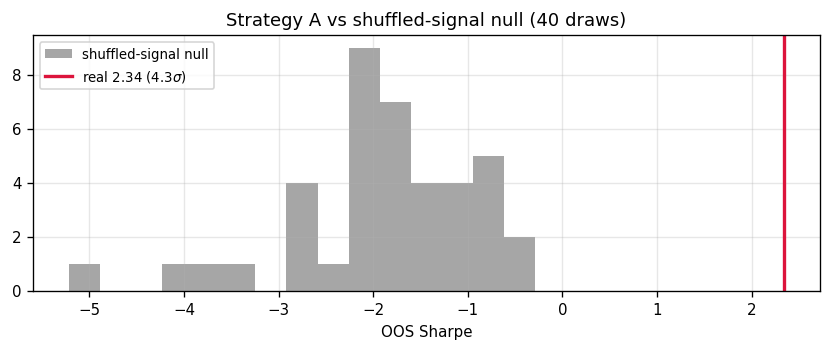
\includegraphics[width=\linewidth]{figures/an_shuffle.png}
  \caption{\textbf{Shuffled-signal null.}  Shuffling the funding signal in time
           destroys the edge (null mean $-1.92$); the real strategy ($2.34$) is
           $+4.3\sigma$ above the null, so timing, not structure, drives the
           alpha.}
  \label{fig:shuffle}
\end{figure}

\subsection{A bootstrap interval for Strategy A}

A block bootstrap gives A a mean Sharpe of $2.39$ and a 95\% range of
$\mathbf{[1.23, 3.70]}$ (Figure~\ref{fig:Aboot})---all positive, but wide, because I
have only one six-month sample.

\begin{figure}[htbp]
  \centering
  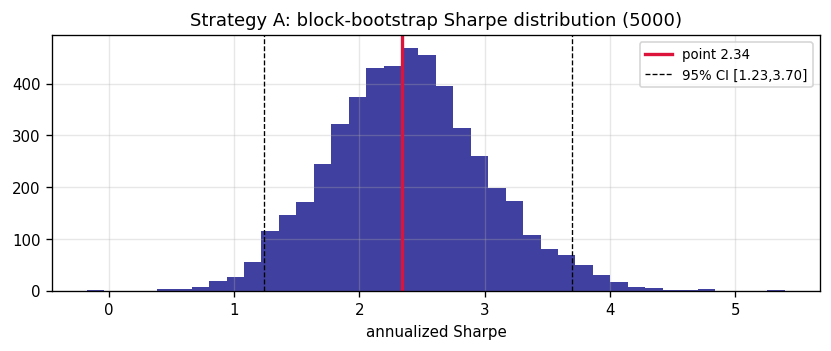
\includegraphics[width=\linewidth]{figures/an_A_bootstrap.png}
  \caption{\textbf{Strategy A: block-bootstrap Sharpe distribution.}  Five thousand
           five-day-block resamples give a mean of $2.39$ and a 95\% range of
           $[1.23, 3.70]$; fully positive but wide, from the single six-month
           sample.}
  \label{fig:Aboot}
\end{figure}

\subsection{The deflated Sharpe ratio}

The hardest test is the deflated Sharpe \cite{bailey2014deflated}, wich counts the
twenty variants I tried.  The benchmark is the highest Sharpe that luck alnoe can give,
\begin{equation}
  \widehat{SR}_0 = \sqrt{\widehat{V}}\left[(1-\gamma_E)\,Z^{-1}\!\Big(1-\tfrac1N\Big)
                 + \gamma_E\,Z^{-1}\!\Big(1-\tfrac{1}{N e}\Big)\right],
  \label{eq:dsr}
\end{equation}
which is about $1.71$ ($N=20$).  So the deflated Sharpe is $\mathbf{DSR \approx 0.68}$
(Table~\ref{tab:dsr}), below the usual $0.95$ bar.  To be honest, on onne six-month
window and twnety trials, teh $2.34$ is only a hint, not clearly significant  The
cross-sectional evidence is strong, but the time-series evidence needs more data.

\begin{table}[htbp]
  \centering
  \caption{\textbf{Deflated Sharpe ratio for Strategy A.}}
  \label{tab:dsr}
  \begin{tabular}{lr}
    \toprule
    \textbf{Quantity} & \textbf{Value} \\
    \midrule
    Annualised Sharpe              & 2.34 \\
    Trials $N$                     & 20 \\
    Return skewness                & $+1.82$ \\
    Return kurtosis                & 42.3 \\
    Deflated benchmark $\widehat{SR}_0$ & 1.71 \\
    PSR against zero               & 0.96 \\
    \textbf{Deflated Sharpe (DSR)} & \textbf{0.68} \\
    \bottomrule
  \end{tabular}
\end{table}

\subsection{Stability as the sample grows}

The expanding-window Sharpe goes to $2.35$ and stays in $[2.2, 3.0]$ after ten weeks
(Figure~\ref{fig:expanding}), so it does not go to zero, and it is not from one lucky
peirod.  A holds a profitable position only $51\%$ of the time, so the return comes
from the skew, not from the hit rate.

\begin{figure}[htbp]
  \centering
  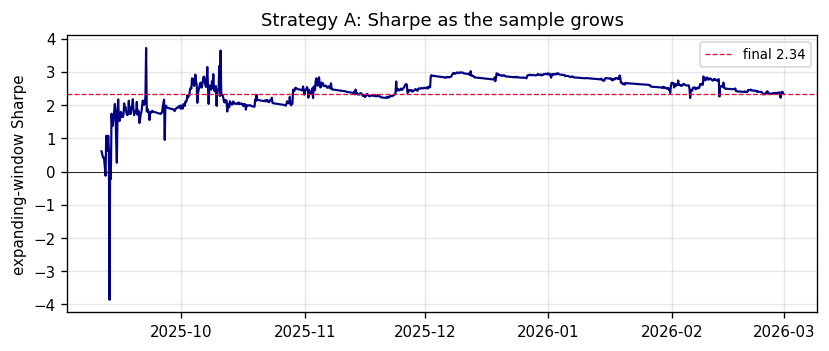
\includegraphics[width=\linewidth]{figures/an_A_expanding.png}
  \caption{\textbf{Strategy A: expanding-window Sharpe.}  The estimate converges to
           $2.35$ and stays within $[2.2, 3.0]$ after the first ten weeks: stable as
           data grow, not decaying or spiking.}
  \label{fig:expanding}
\end{figure}


%% =====================================================================
\section{Portfolio Construction and Production Estimate}
\label{sec:production}
%% =====================================================================

A and B are almost uncorrelated ($-0.03$), so they fit together
(Figures~\ref{fig:ABscale},~\ref{fig:ABdist}): A is low and always on, B is high and
on-off.

\begin{figure}[htbp]
  \centering
  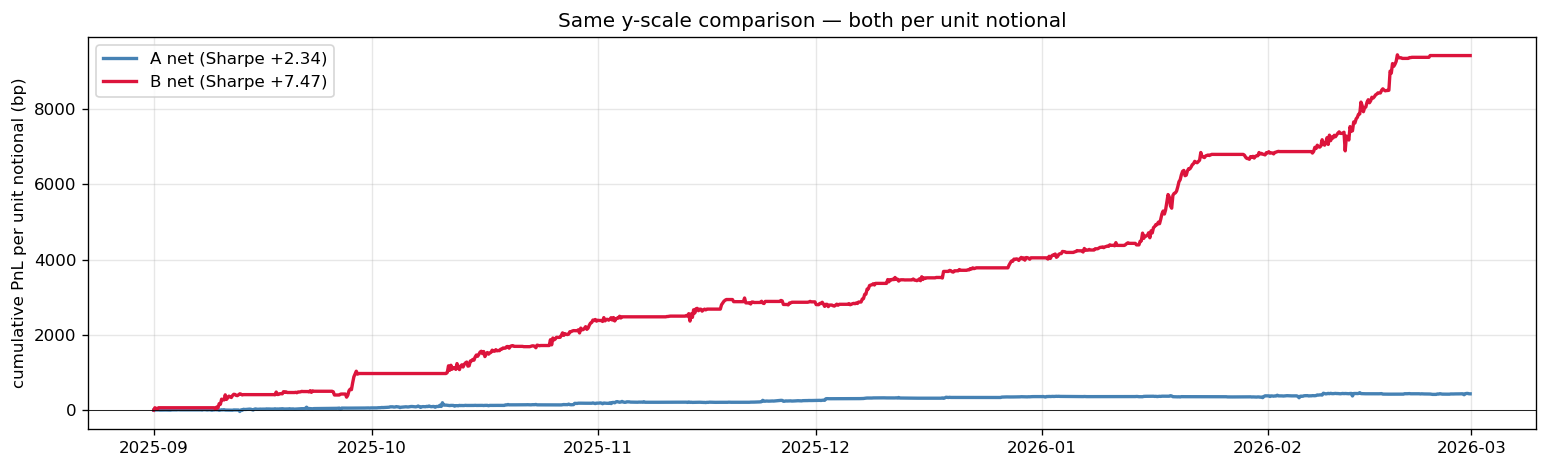
\includegraphics[width=\linewidth]{figures/final_07_AB_same_scale.png}
  \caption{\textbf{Strategies A and B on the same scale.}  A is a steady
           low-amplitude engine; B is on-off and high-amplitude.  Their near-zero
           correlation ($-0.03$) makes them complementary.}
  \label{fig:ABscale}
\end{figure}

\begin{figure}[htbp]
  \centering
  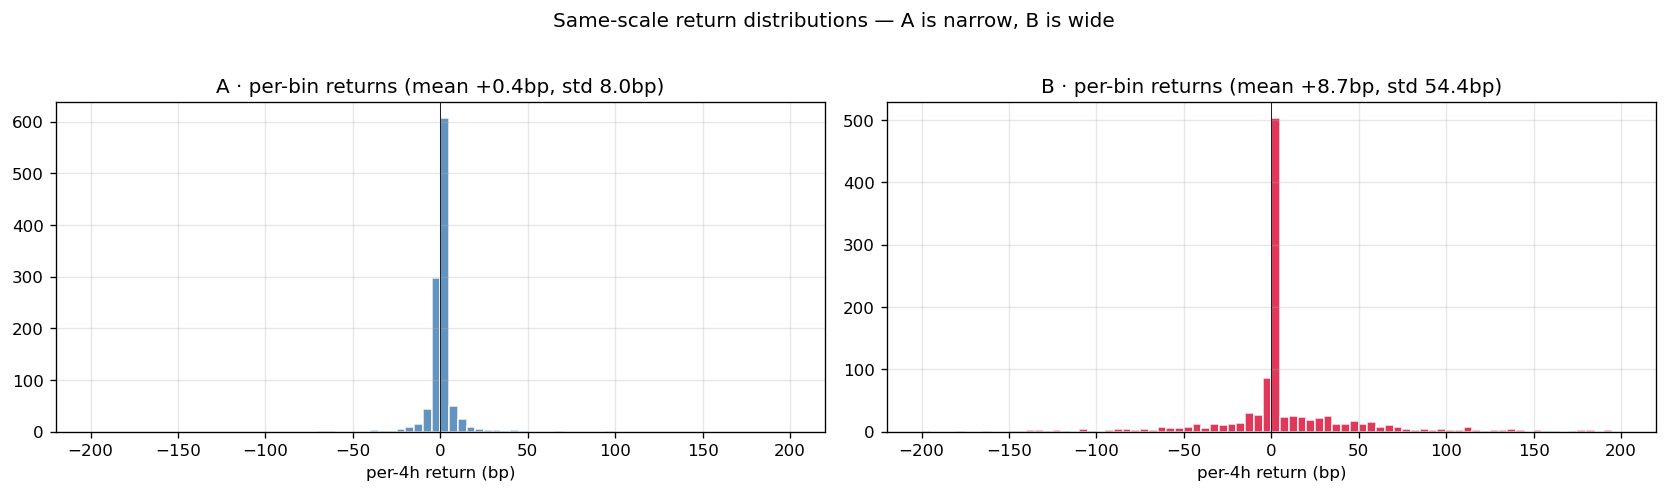
\includegraphics[width=\linewidth]{figures/final_08_AB_return_dist.png}
  \caption{\textbf{Return distributions, A versus B.}  The two strategies sit in
           different parts of return space, so they are distinct trades, not two
           views of one signal.}
  \label{fig:ABdist}
\end{figure}

A naive 70/30 gives tangency a combined Sharpe near $8.0$
(Figure~\ref{fig:ABcombined}), but this number carries all of B's weakness, so it is
only an illustration, not a target.

\begin{figure}[htbp]
  \centering
  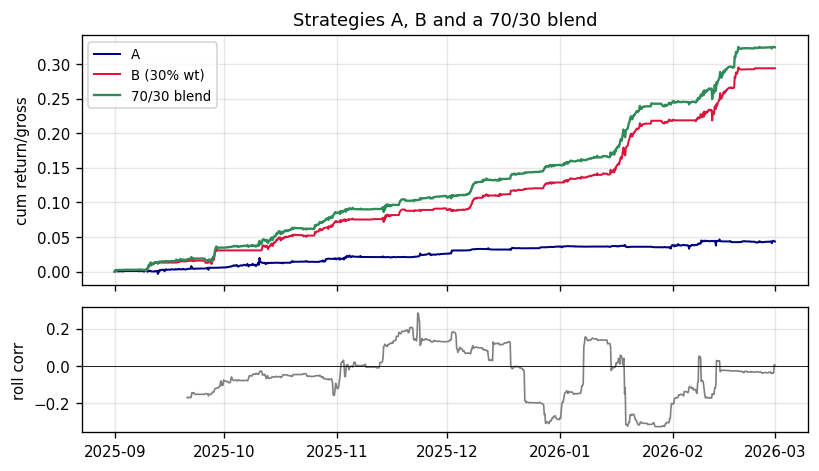
\includegraphics[width=\linewidth]{figures/an_AB_combined.png}
  \caption{\textbf{Strategies A, B and a 70/30 blend.}  The rolling correlation
           (bottom) stays near zero, so the blend's equity is smoother than either
           leg; the in-sample blend Sharpe of $8.0$ is an illustration, not a
           target.}
  \label{fig:ABcombined}
\end{figure}

honest The picture (Table~\ref{tab:production}) is a barbell: A is the main scalable
strategy (a robust $2.34$, any size), and B is a small, capacity-limited one
($[2.41, 3.81]$, but only up to \$130{,}926).

\begin{table}[htbp]
  \centering
  \caption{\textbf{Production estimate.}}
  \label{tab:production}
  \begin{tabular}{lll}
    \toprule
    & \textbf{Strategy A} & \textbf{Strategy B} \\
    \midrule
    Mechanism      & cross-ex pair    & neg.\ carry \\
    Sources        & funding $+$ basis & funding \\
    OOS Sharpe     & 2.34             & 7.47 (in-regime) \\
    Long-run Sharpe& 2.34             & 3.0 $[2.41,3.81]$ \\
    Capacity       & any scale        & \$130{,}926 \\
    Binding risk   & execution        & capacity $+$ regime \\
    Role           & scalable core    & satellite \\
    \bottomrule
  \end{tabular}
\end{table}

A real deployment uses the controls in Table~\ref{tab:checklist}, and each one is tied
to a risk this report measured.

\begin{table}[htbp]
  \centering
  \caption{\textbf{Deployment controls.}}
  \label{tab:checklist}
  \begin{tabular}{ll}
    \toprule
    \textbf{Control} & \textbf{Risk addressed} \\
    \midrule
    Per-coin cap ($\le$5\% cap.)   & coin blow-up \\
    Per-venue cap ($\le$20\%)      & counterparty \\
    Tier-3 total cap ($\le$50\%)   & dead-coin exposure \\
    Spot $-30\%$/1h auto-flatten   & rug pull \\
    Daily $-2\%$ circuit breaker   & drawdown \\
    Monthly walk-forward retrain   & universe drift \\
    Borrow $>$15\% USDC hedge      & financing stress \\
    \bottomrule
  \end{tabular}
\end{table}


%% =====================================================================
\section{Economic Interpretation}
\label{sec:econ}
%% =====================================================================

Why does this edge exist, and why is it not taken away by other people?  In my
understanding, two the strategies are not easy money.  I can earn thhe return because
I tke a risk that other people do not want to take.  Two ideas can explain it: carry
is a kind of risk premium \cite{koijen2018carry}, and arbitrage has its limits
\cite{shleifer1997limits}.

\subsection{Where the return comes from}

In Strategy~A, I am like a person standing between two venues.  On one venue there
are too many longs and on the other venue there are too many shorts, so both sides
pay funding to me.  In Strategy~B, the retail longs on the meme cins are too
crowded, so they pay a high funding to keep their position, and I take the other
side.  So the return is not from prediction.  It is from giving the side that is
missing.  This is also teh reason why the machine-learning model did not help.

\subsection{The risks I take}

As \cite{koijen2018carry} say, carry can earn a premium because it loses money in
bad times.  My strategies also take some risks like tis.  When a coin drops very
fast, the hedge may break (Table~\ref{tab:blowup}).  The borrow cosst may rise very
high, or the pool may be used up, just when the trade wants to grow
\cite{brunnermeier2009market, frazzini2014betting}.  The carry is also closed for
most of the time \cite{schmeling2023crypto}.  And if fails OKX one time, the whole B
book can be lost.  The return is the price I get for taking these risks.

\subsection{Why the cross-exchange spread persists}

To close A's spread, I need to put margin on two, venues at the same tmie, and this
money cannot be shared.  So the gap closes very slowly and stays for a long tiime
\cite{makarov2020trading}; this is the crypto version of capital that moves slowly
\cite{duffie2010presidential}.  In simple words, the spread is the money I get for
putting capital on two venues at the same time, and this is also why the trrade
cannot be too large---it is limited by depth.

\subsection{Why deeply-negative funding persists}

To get B's carry, I must short the spot, and to short the spot I must borrow the
coin.  But for these small coins, the amount I can borow is very small, only about
\$130k (Table~\ref{tab:capacity}), and the rate is high.  So no one can do this trade
in a large size, and the negative, funding do not go awy.  The borrow limit is
exactly the limit to arbitrage \cite{frazzini2014betting}.

\subsection{Benchmarking against the literature}

Other crypto papers report a Sharpe of about $1$--$2$
\cite{liu2022common, schmeling2023crypto} (Table~\ref{tab:bench}).  My Strategy~A
($2.34$) and Strategy~B ($\approx 3$) are higher, but the main reason is that they
are narrower and have smaller capacity.

\begin{table}[htbp]
  \centering
  \caption{\textbf{Benchmarking against published crypto strategies.}}
  \label{tab:bench}
  \begin{tabular}{lrl}
    \toprule
    \textbf{Strategy} & \textbf{Sharpe} & \textbf{Capacity} \\
    \midrule
    Liu--Tsyvinski--Wu factors  & 1--2  & broad \\
    Crypto carry (Schmeling)    & 1--2  & broad \\
    Strategy A (this work)      & 2.34  & any scale \\
    Strategy B (this work)      & $\sim$3 & \$130k \\
    \bottomrule
  \end{tabular}
\end{table}


%% =====================================================================
\section{Implementation Considerations}
\label{sec:impl}
%% =====================================================================

A backtest is only a hypothesis, not the real system.  Below I write what a real
deployment needs.

\subsection{Execution}

Both strategies, make a decision every 4 hours, but inside teh bin the order should be
done slowly, maker first.  This is the most important for Strategy~A, because it only
breks even near $2.7$~bp; if I pay the taker spread, the Sharpe falls from about
$2.3$ to about $1$.  Strategy~B is easier here, but it has one more problem: I must
borrow the coin for the short leg.

\subsection{Monitoring}

Every risk should have a live monitor: close the position automatically when a coin
drops fast, a cap for each venue, a check on the borrow rate, a tracker for the
regime, and a daily stop-loss.

\subsection{Operational and custody risk}

The biggest loss is not from the market but from operation: if one exchange, fails,
the whole B book can be lost.  Strategy~B earns only about \$50k per year, but it can
lose \$130k in one event.  So the main job is to spread the money across exchanges
and counterparties, not to improve the signal.

\subsection{A staged go-live plan}

I would not use the full size directly, from the backtest.  The plan have several
steps: first a paper test to check the real fills, then a small-money test below the
B cap, and only after that scale up Strategy~A (Strategy~B cannot scale).  Every step
has a fixed target to pass.


%% =====================================================================
\balance
\section{Limitations}
\label{sec:limits}
%% =====================================================================

I list my main worries, the most serious one first.

\emph{Execution.}  Strategy~A's $2.34$ uses the average price inside the bin; if I
use only one single price, it falls to about $1.4$.  My fill assummption ($0.8$) is
also too simple.

\emph{Only one regime and one year.}  The out-of-sample period is only six months,
and crypto carry depends a lot on teh regime, so another year may be very different.

\emph{Too many trials.}  Because I tried many variants, after the correction
Strategy~A's Sharpe falls to $0.68$ (below $0.95$).  So the $2.34$ is only a hint,
not a sure result, the and way to fix it is more data not more models.

\emph{Data.}  The 4-hour grid is a little rough, and all the funding data come from
only one source.


%% =====================================================================
\section{Conclusion}
\label{sec:conclusion}
%% =====================================================================

Five points are important.  (1)~The naive funding-rank cross-section is a trap: a
$-2.54$ Sharpe after the prcie is counted.  (2)~The common refinements (ML, more
coins, fifteen variants) all fail out of sample.  (3)~Two delta-neutral trades work:
A (Sharpe $2.34$, scalable) and B (in-regime $7.47$).  (4)~They work for different
reasons, so they fit well together.  (5)~B's big number is mainly about regime and
capacity: an honnest long-run Sahrpe of about $3$, inside $[2.41, 3.81]$, and cpped
at \$130k.

One more point: after I correct for the many variants I tried, A's $2.34$ falls to
$0.68$, so it is olny a hint, not a final answer.

In short, I would run A as the main book and B as a small extra, and I would never
use B's $7.47$ as the real expected number.  The main lesson for me is simple: a
funding-only accounting and a full-PnL accounting can be different, by more than
twenty Sharpe points.  For future work, I would check the real fills, use more years
and more data sources, and run a small live test first.


%% -- References -------------------------------------------------------
{\small
\bibliographystyle{IEEEtran}
\nocite{ackerer2024perpetual}
\nocite{makarov2020trading}
\nocite{liu2022common}
\nocite{schmeling2023crypto}
\nocite{foucault2017toxic}
\nocite{almgren2001optimal}
\nocite{moreira2017volatility}
\nocite{borri2022cross}
\nocite{hu2023crypto}
\nocite{sebastiao2021forecasting}
\nocite{bailey2014deflated}
\nocite{newey1987simple}
\nocite{moskowitz2012time}
\nocite{shleifer1997limits}
\nocite{koijen2018carry}
\nocite{brunnermeier2009market}
\nocite{duffie2010presidential}
\nocite{frazzini2014betting}
\bibliography{report_bib}
}

\end{document}
